%\usepackage[a4paper,twoside]{geometry}
\documentclass[a4paper, 10pt]{report}

\usepackage{gensymb}
\usepackage{graphicx}
\usepackage{url}
\usepackage{verbatim} 
\usepackage{amsmath}
\usepackage{subfigure}
\usepackage{amsthm}

%force all images into their own section
\usepackage[section]{placeins}

%schrijf wat je had willen lezen toen je met het rapport begon.
%(Arnoud)

\title{Hough-transform based map stitching after localization uncertainty}
\date{August something, 2012}
\author{Okke Formsma\\University of Amsterdam}

\begin{document}
\maketitle

\chapter*{Abstract}
\addcontentsline{toc}{chapter}{\numberline{}Abstract}
%!TEX root = ../report.tex
\chapter*{Abstract}
\addcontentsline{toc}{chapter}{\numberline{}Abstract}

Robots deployed for Urban Search And Rescue need be able to simultaneously perform mapping tasks and localize themselves, known as the SLAM problem. Most current methods perform 2D laser scan matching to incrementally build a map. When traditional scanmatching methods fail, post-processing can be applied to join the resulting submaps into a coherent whole. 

In this report the results of Hough-transform based map stitching (HTMS) is analyzed on a number of datasets recorded in the USARSim simulation environment, which were split up at points where the scanmatcher failed. Three methods to identify scanmatching failures are compared.

It was found that the HTMS method as presented does not yield better maps than existing scanmatching methods. In indoor environments the rotation estimate given by the HTMS is accurate, but the translation estimate performance is below par. Suggestions for improvements are provided to guide future research.

%!TEX root = ../report.tex
\chapter*{Acknowledgements}
Thanks Arnoud, etc.
Thanks Julian?
Thanks Magda?

\tableofcontents
\pagenumbering{arabic}

The Simulatenous Localization And Mapping (SLAM) method employed by the AJORF (Amsterdam-Oxford Joint Rescue Forces <<cite team description paper>> is not robust against severe tilting of the laser scanner. 

In this report, an extension to the algorithm is proposed which prevents the addition of patches to the map when the laser scanner data is in a plane too far from the horizontal
%!TEX root = ../report.tex

One of the goals of the USAR challenge was to create a useable map of the environment. 

The problem an agent faces when it needs to find it's way in an unknown environment is called SLAM, for Simulatenous Localization and Mapping. The agent has no map of the environment, and also no way of knowing it's exact location. It needs to infer the map and it's position on the map from the information it gathers from it's sensors throughout time.

Thus, SLAM is a chicken-and-egg problem: without a map it is hard to estimate the agent's position, and without the agent's position it's hard to estimate the map!

In this section we will first examine how the robot keeps track of the state of the world, and then how the SLAM problem can be solved with Extended Kalman Filters. 

\subsection{State}
The state of the world as it is known to the agent is denoted $x$. The value of this set of variables may change over time, as the agent collects sensor data from the environment. The state at time $t$ is denoted $x_{t}$. 

Many variables may be included in the state variable $x$. For the purpose of this work, we will assume that it contains at least the agent's \em{pose} and a \em{map of the environment}. 

In most SLAM approaches, two types of sensor data is collected: \em{environmental measurement data} and \em{control data}. Environmental measurement data collects information about the environment, while control data collects information about the robot within the environment. Environmental measurement data  is denoted $z$ (at a specific point in time $z_{t}$). Examples of environmental sensors available to an agent are laser scanners, sonars and video cameras. Control data and GPS signals. Control data sensors collect information intrinsic to the agent: it's velocity and position. Examples of control sensors are odometry sensors, inertia sensors and global positioning systems.

For the purpose of this paper we are mainly interested in the online SLAM problem, in contrast to the full SLAM problem. Online SLAM seeks to estimate the current pose $x_{t}$ and map $m$:

\begin{equation}
p(x_{t}, m | z_{1:t}, u_{1:t})
\end{equation}

In contrast, the full SLAM problem estimates all poses $x$ and map $m$:

\begin{equation}
p(x_{1:t}, m | z_{1:t}, u_{1:t})
\end{equation}

In practice, the difference is that the full SLAM problem reconsiders the location of all previous poses in estimating the map, while online SLAM treats these as given. The full SLAM problem is computationally much more expensive. Thus for time sensitive applications, such as real time robot control, usually only online SLAM is performed.





\subsection{Gaussian filters}


\subsection{Localization}


\subsection{Extended Kalman Filters}

\subsection{ManifoldSLAM}


\subsection{2D slam in 3D environment}
Only a slice of the world is returned - so we need to make sure we are horizontal. Otherwise, the scanner returns wrong readings.


UNCERTAINTY MEASURE BY ARNOUD:
To see if the reduced correlation distance also improves the robustness of
the scan matcher the uncertainty measures returned by the algorithms were
analyzed. This uncertainty measure is the full 3-by-3 covariance matrix of the
Gaussian distribution over the displacement estimate and does not lend itself well
for charting in its original form. Therefore we took the on-diagonal elements that
describe the independent uncertainty in x and y direction and combined these
into a Euclidean distance measure. The trace of the covariance matrix acquired
with Q-WSM is in most cases (94%) smaller than the trace of incremental version. The average uncertainty of the Q-WSM algorithm reduced to 36% of the
average uncertainty of the incremental version.



%!TEX root = ../report.tex

\chapter{Map Stitching with the Hough Transform}
Why hough based?
Alternatives?

[what is map stitching, why is it necessary again?]

Stefano Carpin presented a novel map stitching approach based on the Hough Transform in \cite{carpin2002merging}. It is an extention of the Hough transform which Censi et al. introduced as the \emph{Hough spectrum} \cite{censi2005scan}. Censi et al. used the hough spectrum for a novel scan matcher. 

Remember from the SLAM section (\ref{state}) that aligning two maps takes two parameters: the rotation angle $\theta$ and translation vector $t = [x, y]^T$. The Hough spectrum is used for finding the rotation $\theta$ between a scan and reference map. The implementations of Carpin and Censi et al. diverge in their method of finding the translation vector $t$ between two scans. First, we'll look at what the Hough transform and Hough spectrum are. Then, we'll take a look at how the best matching rotation $\hat\theta$ is found, and finally we'll examine translation $t$ further.

\section{Hough transform}
The Hough transform is in origin a line detection technique, patented by Paul Hough in 1962\cite{hough1962method}. An improved version, which is presented here, was introduced by Duda and Hart\cite{duda1972use}. The Hough transform is also extended to detect circles, ellipsis and parabolas, and also arbitrary 2D shapes\cite{ballard1981generalizing}.

The Hough transform detects lines in the following manner. A line in Cartesian $(x, y)$ space can be defined by it's angle ($\theta$) and distance from the origin $\rho$:

\begin{equation}
\label{eq:line}
x\cos \theta + y\sin \theta = \rho
\end{equation}

Every point in $(x,y)$ space lies on infinitely many lines satisfying equation~\ref{eq:line}. Every angle $\theta$ has a single accompanying distance from the origin $\rho$. Thus, a point in $(x,y)$ space can be represented in the \emph{Hough domain} $(\theta, \rho)$ as a curve. The locations where many curves intersect in the Hough domain correspond to the lines in the original image; remember that lines correspond to points in the Hough domain. 

Finding the intersection of many curves in the continuous domain is computationally expensive. The discrete Hough transform mitigates this problem by discretizing the Hough domain into bins. Every point in the original image `votes' for each bin it belongs to in $(\theta, \rho)$ representation. The strongest lines stand out as bins with a high number of votes.

There are $n_\theta$ angle-bins, and $n_\rho$ distance bins in discrete Hough transform $\mathcal{HT}$. 

\begin{figure}[ht]
\centering
\subfigure[Two lines]{
	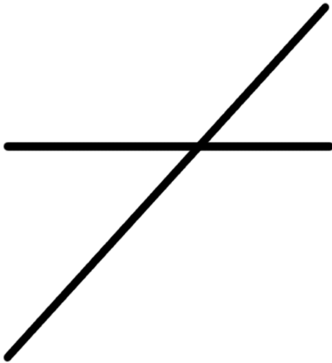
\includegraphics[width=0.4\textwidth]{images/stitching/lines.png}
	\label{fig:lines-original}
}
\subfigure[The Hough transform of \subref{fig:lines-original}]{
	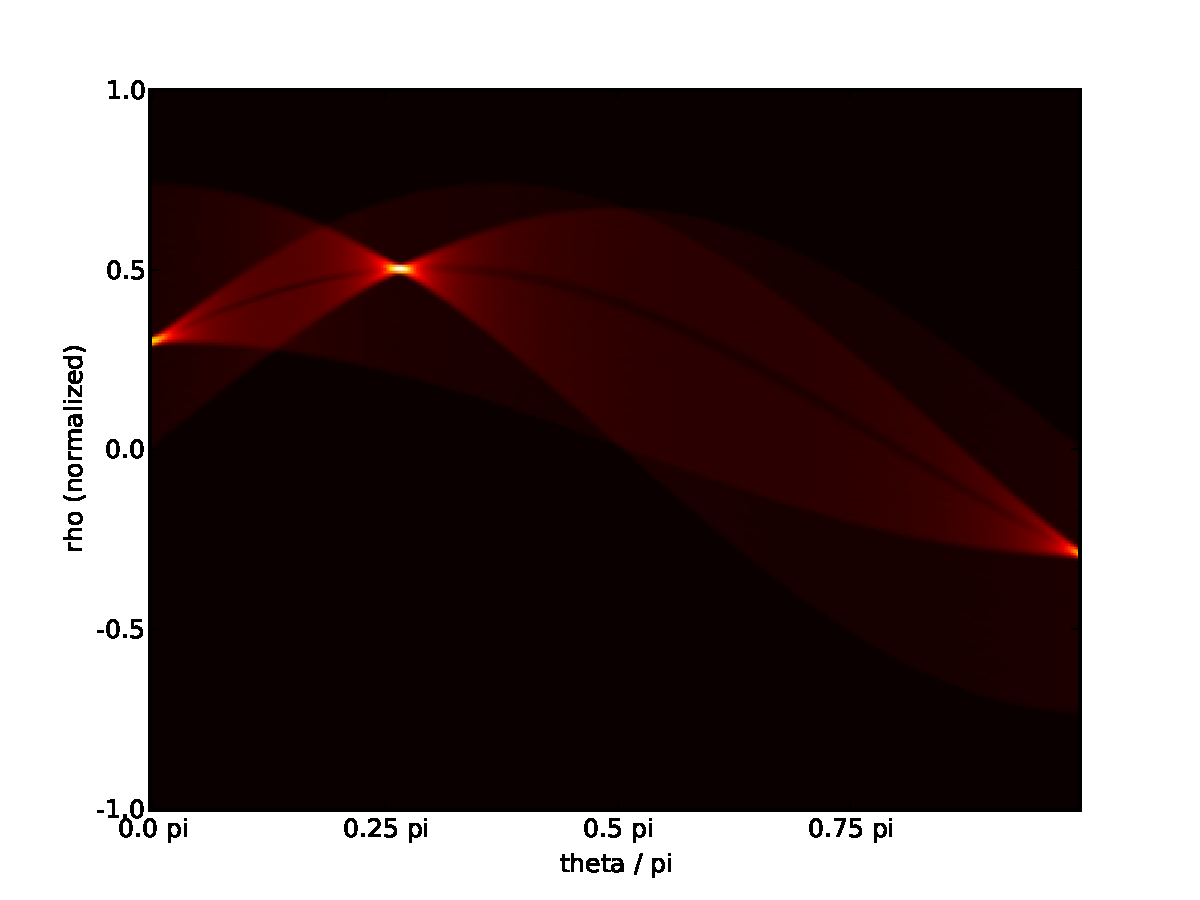
\includegraphics[width=0.55\textwidth]{images/stitching/lines-hough.pdf}
	\label{fig:lines-hough}
}
\caption{Example of the discrete Hough transform. Notice the two maxima in (b) which correspond to the two lines in (a). There seem to be three maxima (one at $0$, one at $\frac{\pi}{4}$ and one at $\pi$). However, the maxima at $0$ and $\pi$ are the same maximum: see section~\ref{sub:periodicity}}
\label{fig:lines}
\end{figure}


\section{Hough spectrum}
The major contribution of Censi et al.\cite{censi2005scan} is the introduction of the Hough spectrum. The Hough spectrum ($\cal HS$) is a measure for the direction of lines in an image. The discrete Hough transform finds the specific lines in the image, while the Hough spectrum finds the most pronounced \emph{directions} of lines in the image:

\begin{equation}
\mathcal{HS}(k) = \eta \sum_{i=1}^{n_\rho} \mathcal{HT} (i, k) ^ 2 \qquad \quad 1 \leq k \leq n_\theta
\end{equation}

$\eta$ is a normalization value to limit $\mathcal{HS}(k)$ to the domain $[0, 1]$.

As we've seen in the previous section, each bin in the discrete Hough transform ($\mathcal{HT} (i, k)$) contains the number of pixels that lie on a line defined by $(\theta_i, \rho_k)$. The hough spectrum is a measure for how strong the lines are on a specific angle. 

Thus, the Hough spectrum yields the highest value in the direction in which the most pronounced lines run. In an indoor environment, there will usually be two peaks, separated by a $90\degree$ angle, corresponding to grid-like structure most buildings are created (see figure~\ref{fig:rooms}). Incidentally, in a bee-hive, with hexagonal chambers, we would see 3 peaks each separated by $60\degree$  angles. See figure~\ref{fig:beehive}.

\begin{figure}[ht]
\centering
\subfigure[A stylistic map of some rooms]{
	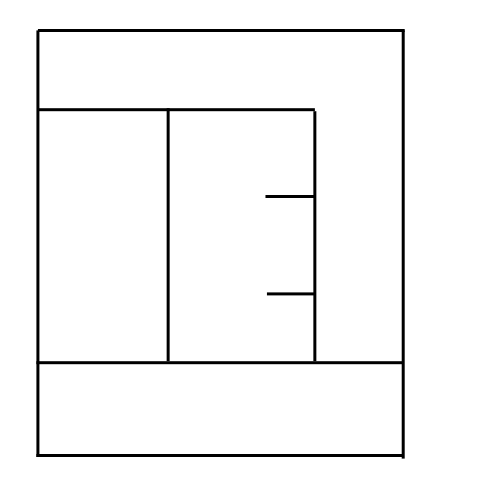
\includegraphics[width=0.4\textwidth]{images/stitching/rooms.png}
	\label{fig:rooms-original}
}
\subfigure[The Hough transform and Hough spectrum of \subref{fig:rooms-original}]{
	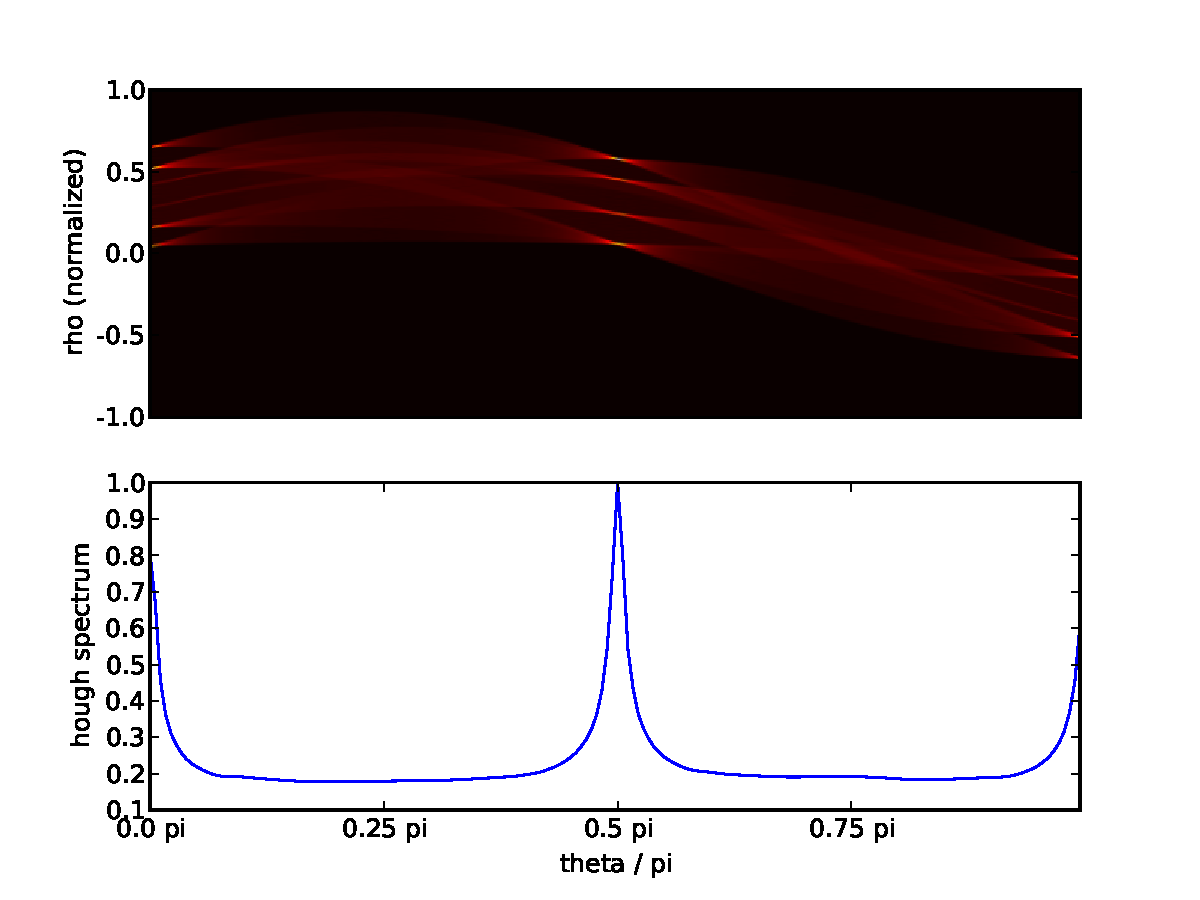
\includegraphics[width=0.55\textwidth]{images/stitching/rooms-hough.pdf}
	\label{fig:rooms-hough}
}
\caption{Example of a hough spectrum in a human-made environment.}
\label{fig:rooms}
\end{figure}

\begin{figure}[ht]
\centering
\subfigure[Hexagonal chambers]{
	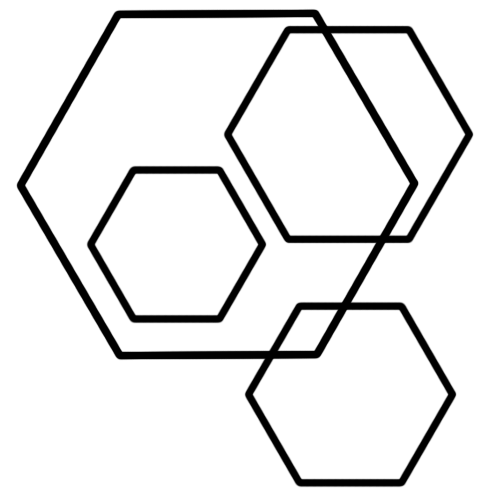
\includegraphics[width=0.4\textwidth]{images/stitching/beehive.png}
	\label{fig:beehive-original}
}
\subfigure[The Hough transform and Hough spectrum of \subref{fig:beehive-original}]{
	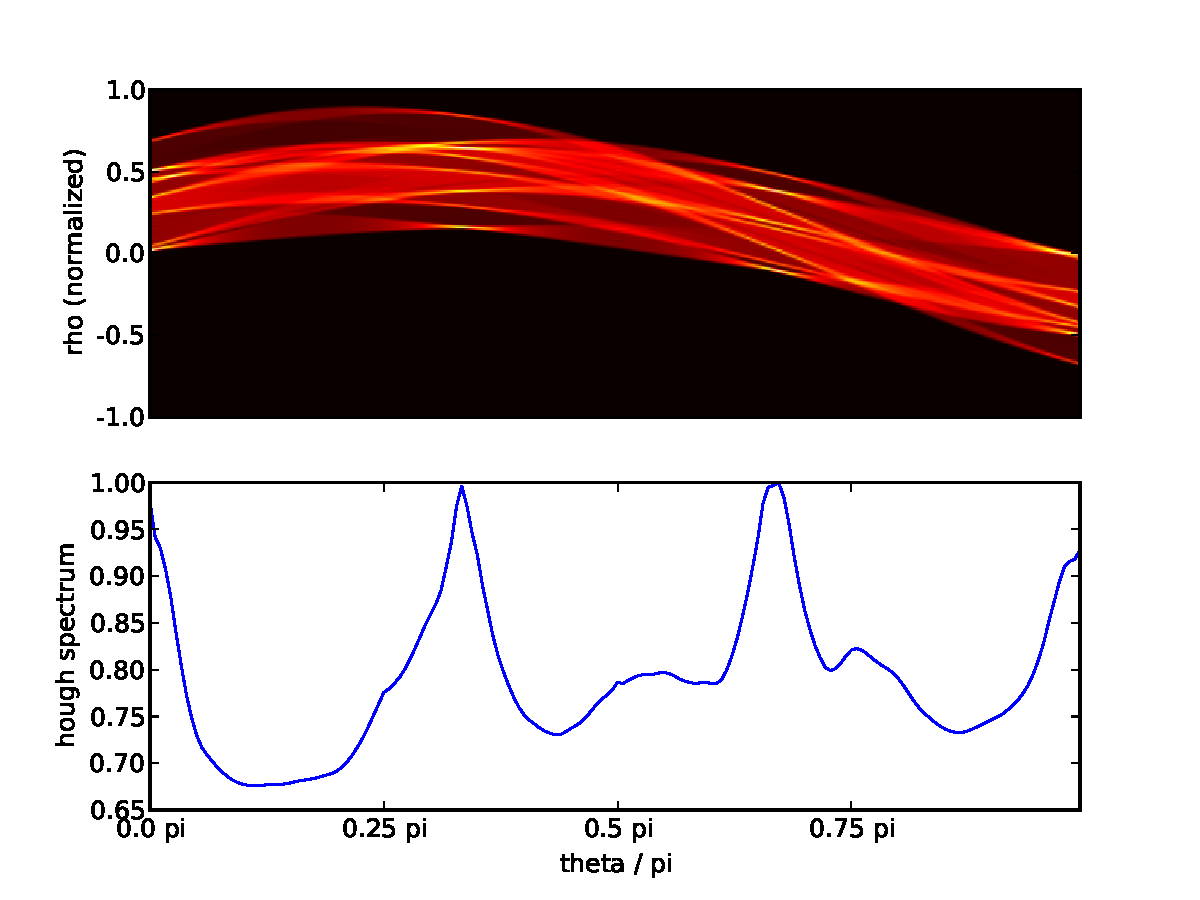
\includegraphics[width=0.55\textwidth]{images/stitching/beehive-lines.pdf}
	\label{fig:beehive-hough}
}
\caption{Example of the Hough spectrum in a hexagonal environment. Notice the three maxima in the Hough Spectrum.}
\label{fig:beehive}
\end{figure}

\section{Finding rotation $\theta$}
Now we can calculate the Hough spectra $\mathcal{HS}_{M_1}$ and $\mathcal{HS}_{M_2}$ for maps $M_1$ and $M_2$. 

\begin{figure}[ht]
	\centering
	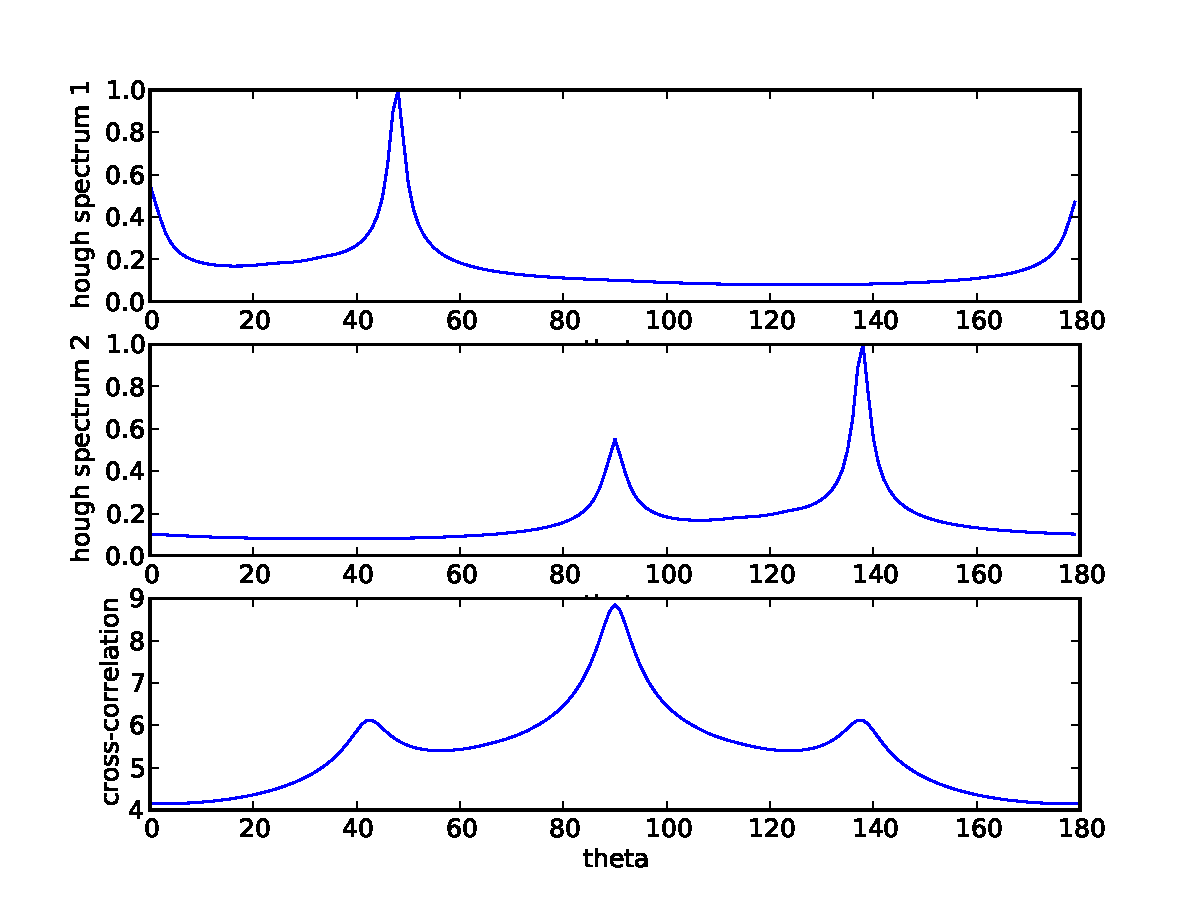
\includegraphics[width=\textwidth]{images/stitching/lines-cross-correlation.pdf}
	\label{fig:lines-cross-correlation}
	\caption{The top two plots are the hough spectra of image~\ref{fig:lines-original}. For the second hough spectrum, it was rotated $90\degree$ counter-clockwise. The cross-correlation shows that the most probable rotation is indeed $90\degree$, with smaller peaks for $45\degree$ and $135\degree$.}
\end{figure}

Notice that the spectra have a periodicity of $180\degree$, and have similar peaks. However, the peaks are at different angles. The cross-correlation of the two signals shows the similarity of the two spectra as one of them is shifted over the x-axis. The cross-correlation $\mathcal{CC}_{M_1,M_2}$ is calculated as follows:

\begin{equation}
\mathcal{CC}_{M_1,M_2}(k) = \sum_{i=1}^{n_\theta} \mathcal{HS}_{M_1}(i) \times \mathcal{HS}_{M_2}(i + k) \qquad 1 \leq k \leq n_\theta
\end{equation}

\subsection{Periodicity}
\label{sub:periodicity}
Why are do the Hough spectra have a periodicity of $180\degree$? The answer lies in the following equations:

\begin{eqnarray}
x\cos \theta + y\sin \theta &=& \rho \\
x\cos(\theta + \pi) + y\sin (\theta + \pi) &=& -\rho
\end{eqnarray}

Thus, the following equation holds: $\mathcal{HT}(\theta_\alpha, \rho_\alpha) = \mathcal{HT}(\theta_\alpha + \pi, -\rho_\alpha)$. In turn, the Hough spectrum of $\theta_\alpha$ and $\theta_\alpha + \pi$ are the same, because $\mathcal{HS}$ is summed over all $\rho$. 

Thus, the domain of $\theta$ only needs to be $[0, \pi)$, whereafter it wraps back to itself. Prior work by Jankowska used the domain $[0, 2\pi\rangle$ \cite{jankowska}, which is thus superfluous.

One must take care when using this representation to remember the possible alternative hypothesis for $\theta$. Every candidate solution $\hat\theta$ found by the cross-correlation method has an additional solution $\hat\theta + \pi$!

\section{Finding translation $t$}
In the previous section we found rotation candidates which align the maps according to the major wall-directions. To find the best match between two maps, we also need to find the optimal translation between them. 

Censi et al.\cite{}

Jankowska (\cite{jankowska2009hough}) takes the same approach as Carpin (\cite{carpin2008merging}). The method is to calculate an X-spectrum and Y-spectrum from the maps and the optimal translation is found by cross-correlating the spectra. We will 


\section{Evaluating stitching results}

\section{Variations on the Hough-transform based stitching}



* Assumption: indoor environment
* Can be used for re-initialization of the manifold method when position is lost! Awesome if a full scan matcher is used after the hough transform based method.
%!TEX root = ../report.tex
\chapter{Method}
\label{method}

In this chapter the design of the experiment is outlined. The experiment consists of three phases: dataset collection, map generation, map segmentation and map stitching. Each of the phases is described in detail below.

\section{Dataset collection}
The dataset for the experiments consists of sensor data acquired by a robot in the USARSim (Urban Search And Rescue Simulation) environment \cite{balaguer2008usarsim, usarsimsite}. USARSim is a high fidelity simulation environment in which reconnaissance and rescue missions can be imitated. These environments can both be indoors and outdoors, and are typically not larger than a housing block. A team of robots is deployed in this environment with the task of localizing (human) victims. One of the goals of the USARSim project is to improve autonomous behavior, allowing one human operator to control a team of up to 16 robots simultaneously.

Much work has been done to increase the realism of the simulation. A selection of recent work: an assessment for use of USARSim in Human Robot Interaction \cite{wang2005validating}, for use with walking robots \cite{van2012validation}, adding realistic laser sensor behavior in environments with smoke \cite{formsma2011realistic} and creating a omnidirectional camera sensor \cite{schmits2009omnidirectional}.

Teams from all over the world compete in the annual RoboCup Rescue Simulation competition \cite{robocupsite}. The universities of Oxford and Amsterdam participated until 2011 with a cooperative team: the Amsterdam Oxford Joint Rescue Forces \cite{aojrf2011, visser2012uva}. The robot control software used by this team is UsarCommander (available on the AOJRF site \cite{jrfsite}). UsarCommander (see figure \ref{fig:usarcommander}) contains a number of SLAM implementations, including ManifoldSLAM.

Three datasets were collected on two recent USARSim maps: the first dataset in a building without smoke, the second two in a larger building. The robot was driven around the map. Care was taken to ensure that the robot visited the same locations a number of times to make the map-stitching method feasible.

Each dataset was recorded. The datasets are available within the code repository \cite{github}.

\section{Map segmentation}
The datasets thus recorded are processed through the UsarCommander ManifoldSlam implementation. At every timestep the scan matcher runs and saves current position and rotation according to the groundtruth, the inertia sensor and the SLAM algorithm, as well as the correspondence error matrix as discussed in section~\ref{scanmatching}.

After creating the map, three uncertainty metrics are evaluated to decide where the map should be segmented. The three metrics are the determinant of the correspondence error, the trace of the correspondence error and the number of matching scans, as discussed in section~\ref{uncertainty}.

The three metrics are manually examined for each map, as we found no prior research in a good metric for map segmentation. Obvious candidates are the maxima in the determinant and trace measures and minima for the number of matching scans. These values are expected to be highly correlated. The dataset is segmented at the thus acquired uncertainty threshold into consecutive parts. For example, if the map consisted of $100$ timesteps ($0 \ldots 99$) and the uncertainty metrics indicate that the highest uncertainty was at timesteps 11, 25 and 70, the dataset is divided into four segments: $0 \ldots 10$, $11 \ldots 24$, $26 \ldots 69$, and $71 \ldots 99$. A submap is generated for each segment.

\section{Map stitching}
The segments are matched according to the Hough-transform based map stitching method as outlined in chapter~\ref{chapter:hough}. In that chapter it is explained that there may be a number of rotation estimates $\hat \theta$. We will assume in the experiment that the smallest absolute rotation candidate $|\hat \theta|$ will be the most probable. This is based on the observation that the scanmatcher usually does not yield very large rotation errors.

The relative X- and Y-positions of the maps are estimated exactly as explained in the map stitching chapter.

\section{Evaluation}
In line with the exploratory nature of this work the maps will not be evaluated using a groundtruth-metric. Instead, manual assessment of the results will yield a qualitative judgment about the quality of the resulting map. The main concern is whether the resulting map is an improvement upon the map provided by the ManifoldSLAM algorithm.
%!TEX root = ../report.tex
\chapter{Experiments}
\label{experiments}
In this chapter the experimental results are presented. The experimental method is outlined in chapter~\ref{method}. 

\section{Experiment 1: IranOpen 2012 - Pre 2 map}
This map was used in the Iran Open 2012 competition \cite{iran2012}. The map features a grey hospital-like environment with grey tiled floors and walls. In figure~\ref{fig:map1} a screenshot of the environment is shown along with the map after the Weighted Scan Matcher was run on the simulation data. 

\begin{figure}[ht]
\centering
\subfigure[Screenshot]{
	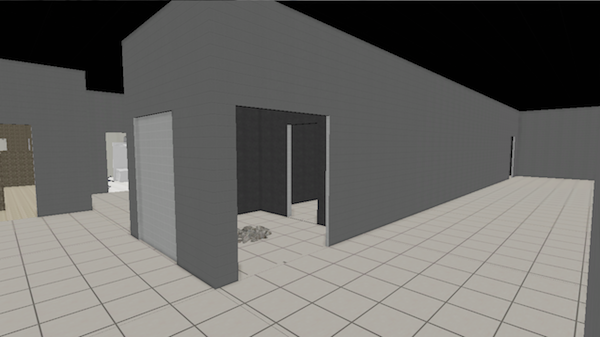
\includegraphics[width=0.5\textwidth]{images/experiment/map1/screenshot.png}
	\label{fig:map1-screenshot}
}
\subfigure[Map created with the Weighted Scan Matcher]{
	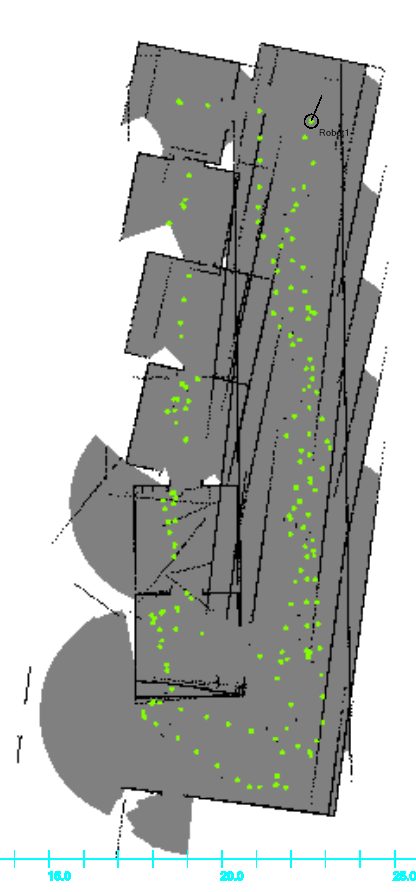
\includegraphics[width=0.3\textwidth]{images/experiment/map1/slam.png}
	\label{fig:map1-map}
}
  \caption{The ground truth, inertia sensor and slam path of the robot on a piece of map 1.}
  \label{fig:map1}
\end{figure}

The map shows a lot of noise and errors. As can be seen in figure~\ref{fig:apx:map1-paths} (in the appendix), the inertia sensor gives a rather good location-estimate, but the rotation estimate from position 160 onwards is off by more than $10\degree$. The scanmatcher fails regularly because it takes the inertia sensor location estimate as begin point for its search. When the location according to SLAM and inertia sensor diverge too far, the SLAM matcher fails -- it only searches a local neighborhood around the initial seed pose given by the inertia sensor. The result of this is a map with jagged lines, as can be seen in figure~\ref{fig:map1-map} and figure~\ref{fig:map1-ins-problem}.

\begin{figure}[ht]
  \centering
  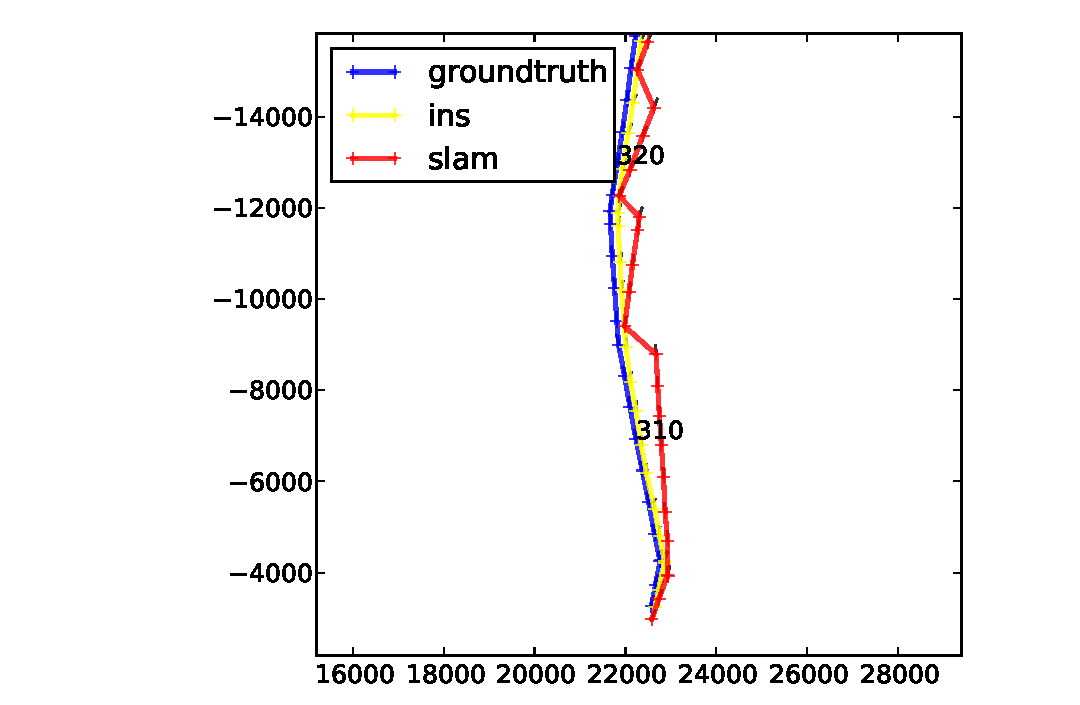
\includegraphics[width=0.7\textwidth]{images/experiment/map1/ins-problem.pdf}
  \caption{A small part of the path the robot moved in map 1. The wrong rotation estimate of the inertia sensor (yellow line) makes the slam-matcher (red line) think the robot moved in another direction than it did in reality (blue line). When the inertia sensor reading and SLAM result diverge too far, the SLAM location is reset to the inertia sensor estimate. This results in a jagged path estimate from the SLAM sensor.}
  \label{fig:map1-ins-problem}
\end{figure}


\subsection{Segmenting the map}
The confidence measures of the first map are shown in figure~\ref{fig:map1-confidence-measures-vs-time}. It is immediately apparent that the extreme values of the three metrics coincide. When the scan matcher matches few scanlines, the determinant and trace values are at their maximum. When the scan matcher matches no scanlines, the determinant and trace of the covariance matrix are undefined. These show up as red dots on the x-axis. When the scan matcher matches many scanlines, its increased confidence in a correct match is reflected in a covariance matrix with small determinant and trace.

In figure~\ref{fig:map1-confidence-measures-scatter} the values of the three confidence measures are plotted against each other to emphasize their correlation. The (Spearman) rank correlation gives an indication how well the relationship between the two variables can be described by a monotonic function. The spearman rank correlation coefficients between the confidence measures is as follows. Between trace and determinant $0.85$, between number of matches and determinant $-0.50$, and between number of matches and trace $-0.48$, all with a p-value $\ll 10^{-10}$. This means that all three confidence measures are strongly correlated.

\begin{figure}[ht]
  \centering
  \subfigure[Confidence measures through time]{
    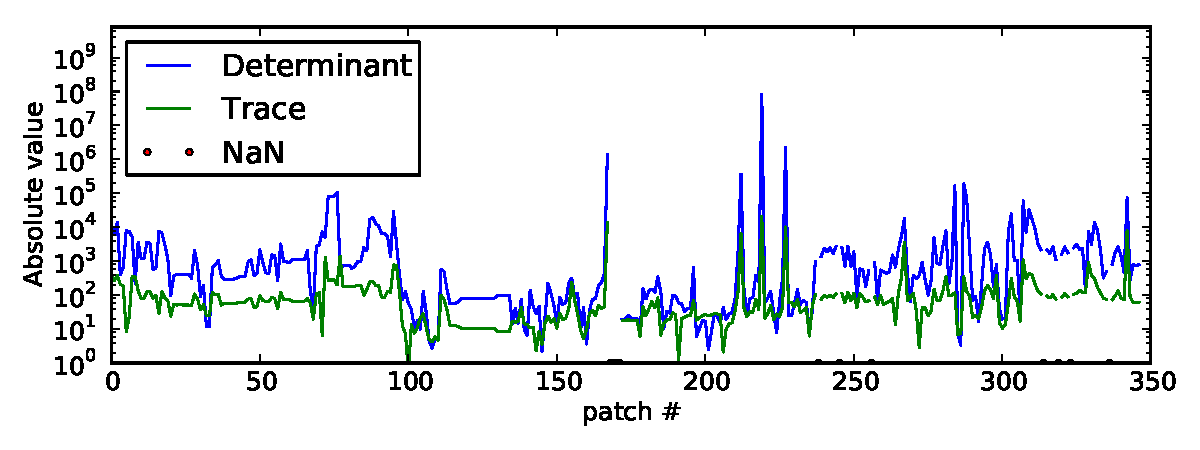
\includegraphics[width=\textwidth]{images/experiment/map1/error-measures.pdf}
    \label{fig:map1-confidence-measures-vs-time}
  }
  \subfigure[Scatter plot between the three confidence measures.]{
    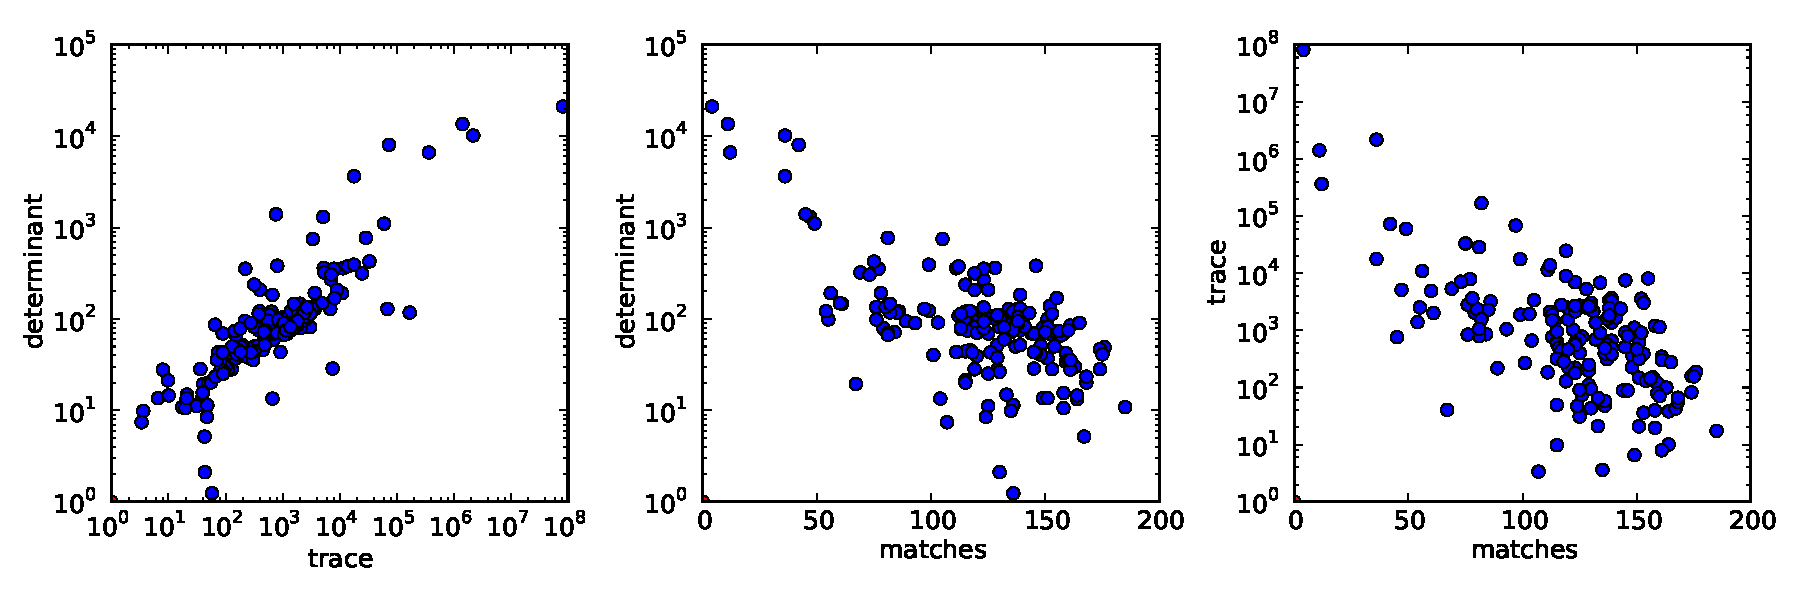
\includegraphics[width=\textwidth]{images/experiment/map1/error-measures-scatter.pdf}
    \label{fig:map1-confidence-measures-scatter}
  }
  \caption{Confidence measures for map 1.}
  \label{fig:map1-confidence-measures}
\end{figure}

When there are no matches at all, the scanmatcher has failed most spectacularly. In that case, the covariance matrix can not even be computed. In extention, the determinant or trace of the covariance matrix can not be computed either. This occurs at the following timesteps: 66  67  68  96 103 113 159 164 168 175. The greatest rift lies at $66 \le t \le68$, where there were 3 consecutive timesteps that could not be matched. The submaps that are procured can be found in the appendix, figure~\ref{fig:apx:map1-pieces}. 

\subsection{Stitching}
The Hough map stitching procedure as outlined in chapter~\ref{chapter:hough} between the first two sub-maps results in an optimal rotation $\theta_1$ of $13\degree$, with a much less pronounced secondary hypothesis $\theta_2$ of $103\degree$, as can be seen in figure~\ref{fig:exp:1:theta}. The X- and Y-spectra for $\theta_{1a}$ are shown in figure~\ref{fig:exp:1:xy}. The resulting map is shown in figure~\ref{fig:exp:1:result1}.

\begin{figure}[ht]
  \centering
  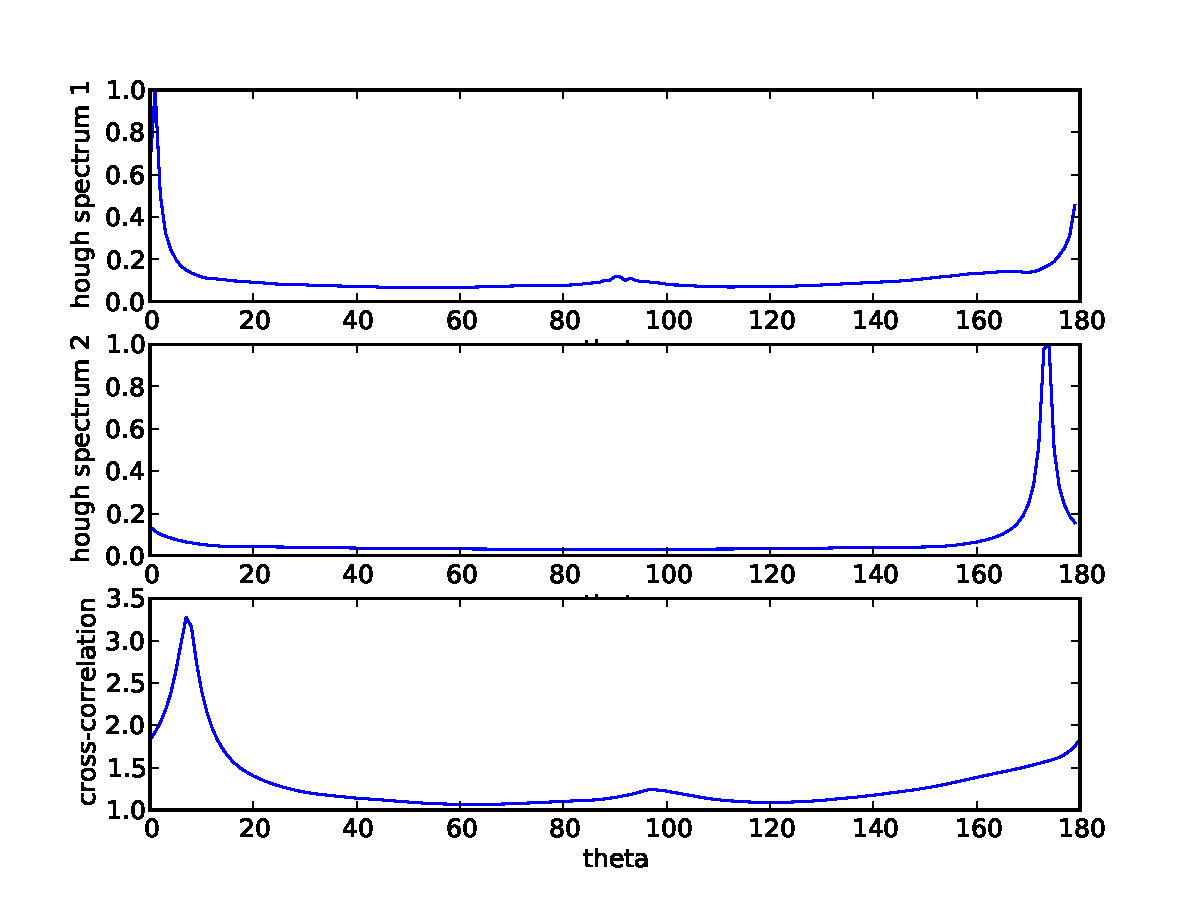
\includegraphics[width=0.8\textwidth]{images/experiment/map1/stitch1-theta-correlation-result.pdf}
  \caption{Finding optimal rotation $\theta$ through correlating Hough spectra.}
  \label{fig:exp:1:theta}
\end{figure}

\begin{figure}[ht]
  \centering
  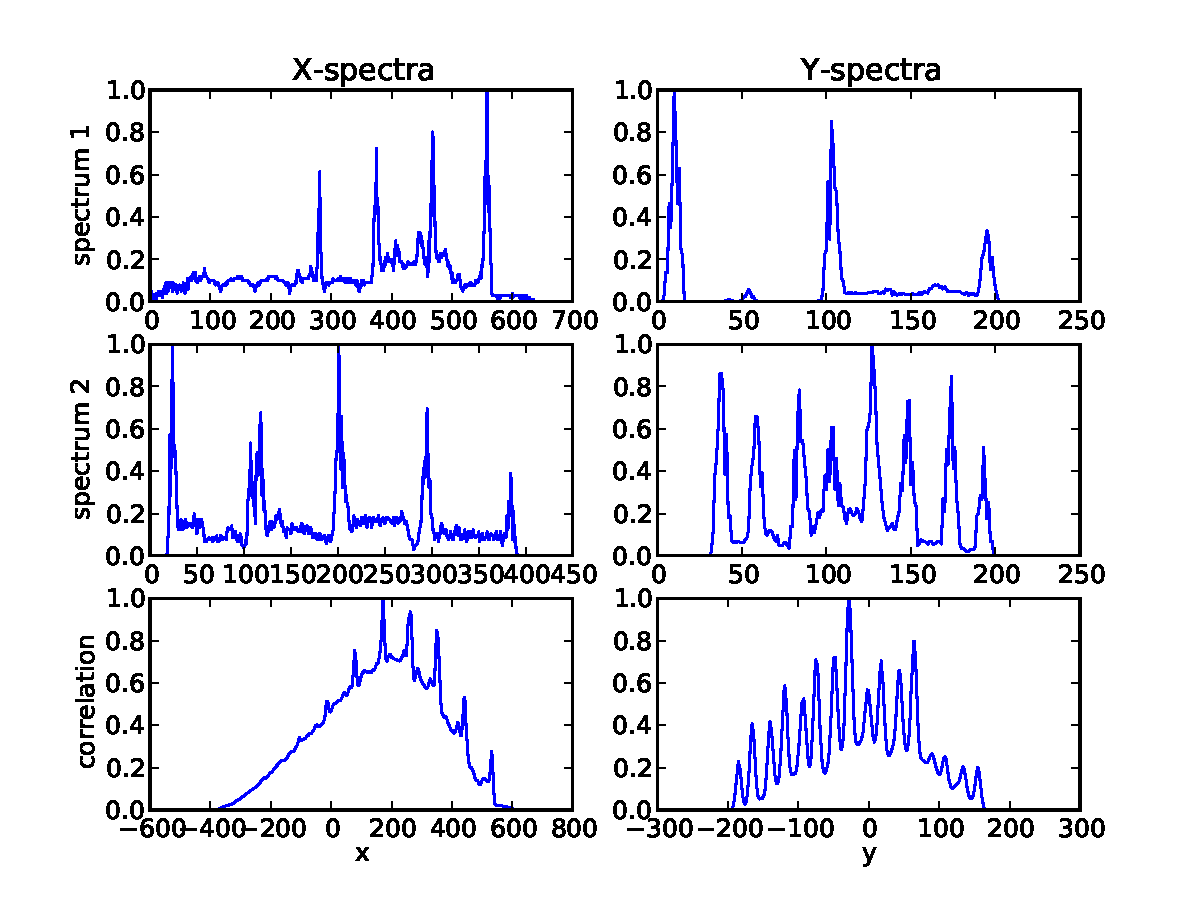
\includegraphics[width=0.8\textwidth]{images/experiment/map1/stitch1-1a-xy-correlation.pdf}
  \caption{Finding optimal translation $t$ through correlating Hough spectra.}
  \label{fig:exp:1:xy}
\end{figure}

\begin{figure}[ht]
  \centering
  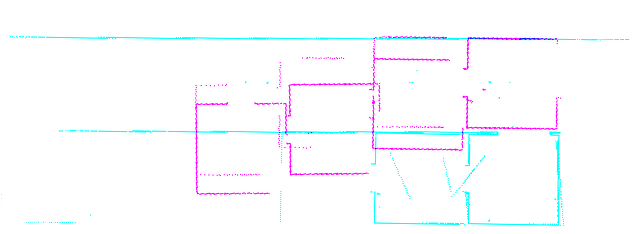
\includegraphics[width=0.8\textwidth]{images/experiment/map1/stitch1-1a-result.png}
  \caption{The best stitch according to $\theta_{1a}$ and optimal $t$.}
  \label{fig:exp:1:result1}
\end{figure}

The result of this stitch is far from optimal. While the rotation angle $\theta_{1a}$ is optimal and the images are rotated correctly, the translation estimate $t$ is very much off. The Hough-transform based map stitching method requires a large overlapping area between the two submaps. Because the submaps overlap very little, the stitching method fails.

In the next figure, \ref{fig:exp:1:result8}, the final result of stitching all submaps in figure~\ref{fig:apx:map1-pieces} is shown. Each of the steps is separately shown in the appendix (\ref{appendix:exp1}).

\begin{figure}[ht]
  \centering
  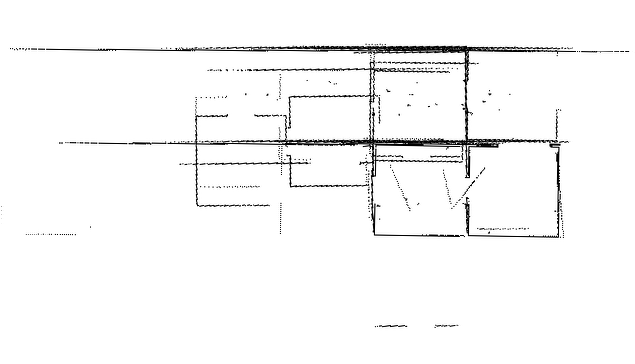
\includegraphics[width=0.8\textwidth]{images/experiment/map1/result/step8.png}
  \caption{The result of stitching all partial maps (see figure~\ref{fig:apx:map1-pieces}) according to the Hough stitching method. Compare to the original SLAM result, figure~\ref{fig:map1-map}.}
  \label{fig:exp:1:result8}
\end{figure}

\section{Experiment 2: IranOpen 2012 Semifinal map with smoke (I)}
The second map is again a map from the IranOpen 2012 championship. The map was used for the semi-final. It is rather large, and consists of many corridors and rooms filled with desks, chairs and computers. Some of the hallways are obstructed, and there is smoke everywhere. See figure~\ref{fig:map3-screenshot}.

\begin{figure}[ht]
\centering
  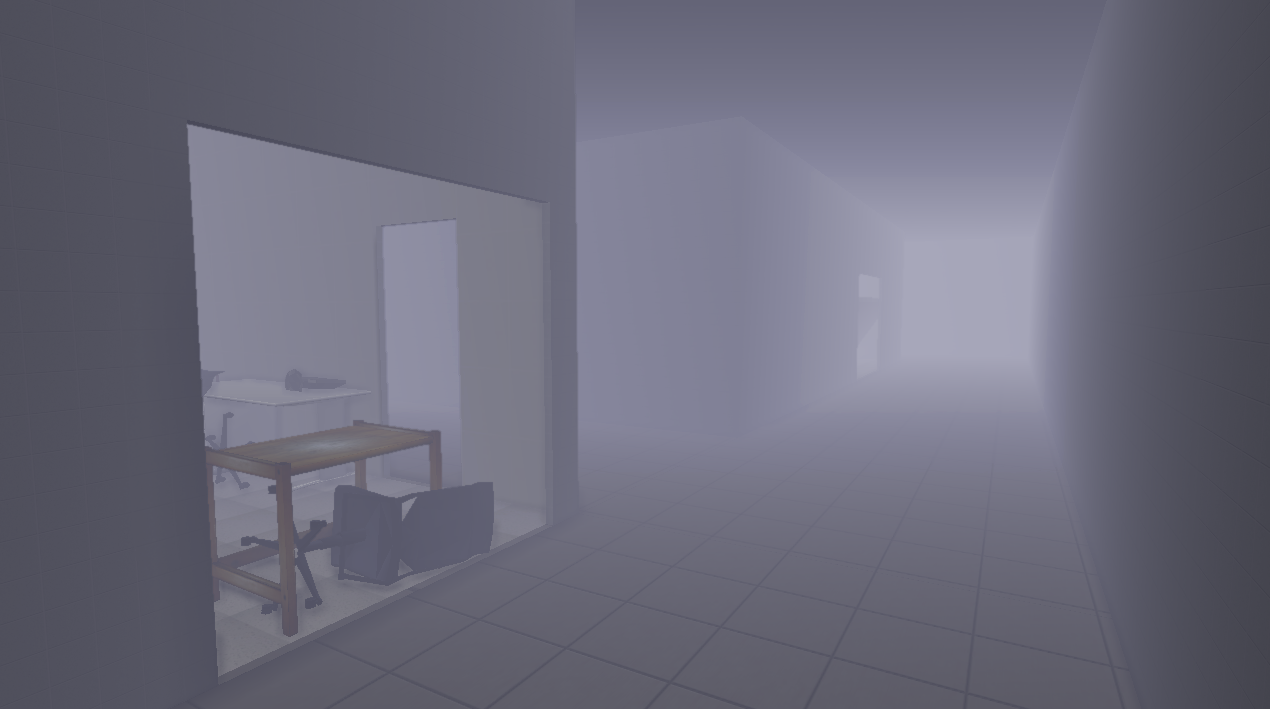
\includegraphics[width=0.5\textwidth]{images/experiment/map3/map3.png}
  \caption{A screenshot of map 2.}
  \label{fig:map3-screenshot}
\end{figure}

The agent was driven in a large circular path ($50m$ diameter) through the building, as can be seen in figure~\ref{fig:map3-trace}. Again, the path given by the inertia sensor seems to lie closer to the groundtruth than the SLAM path. The SLAM path strays on many places from the path by the inertia sensor and SLAM, and is `pulled back' to the location given by the inertia sensor when the difference becomes too large.

\begin{figure}[ht]
\centering
  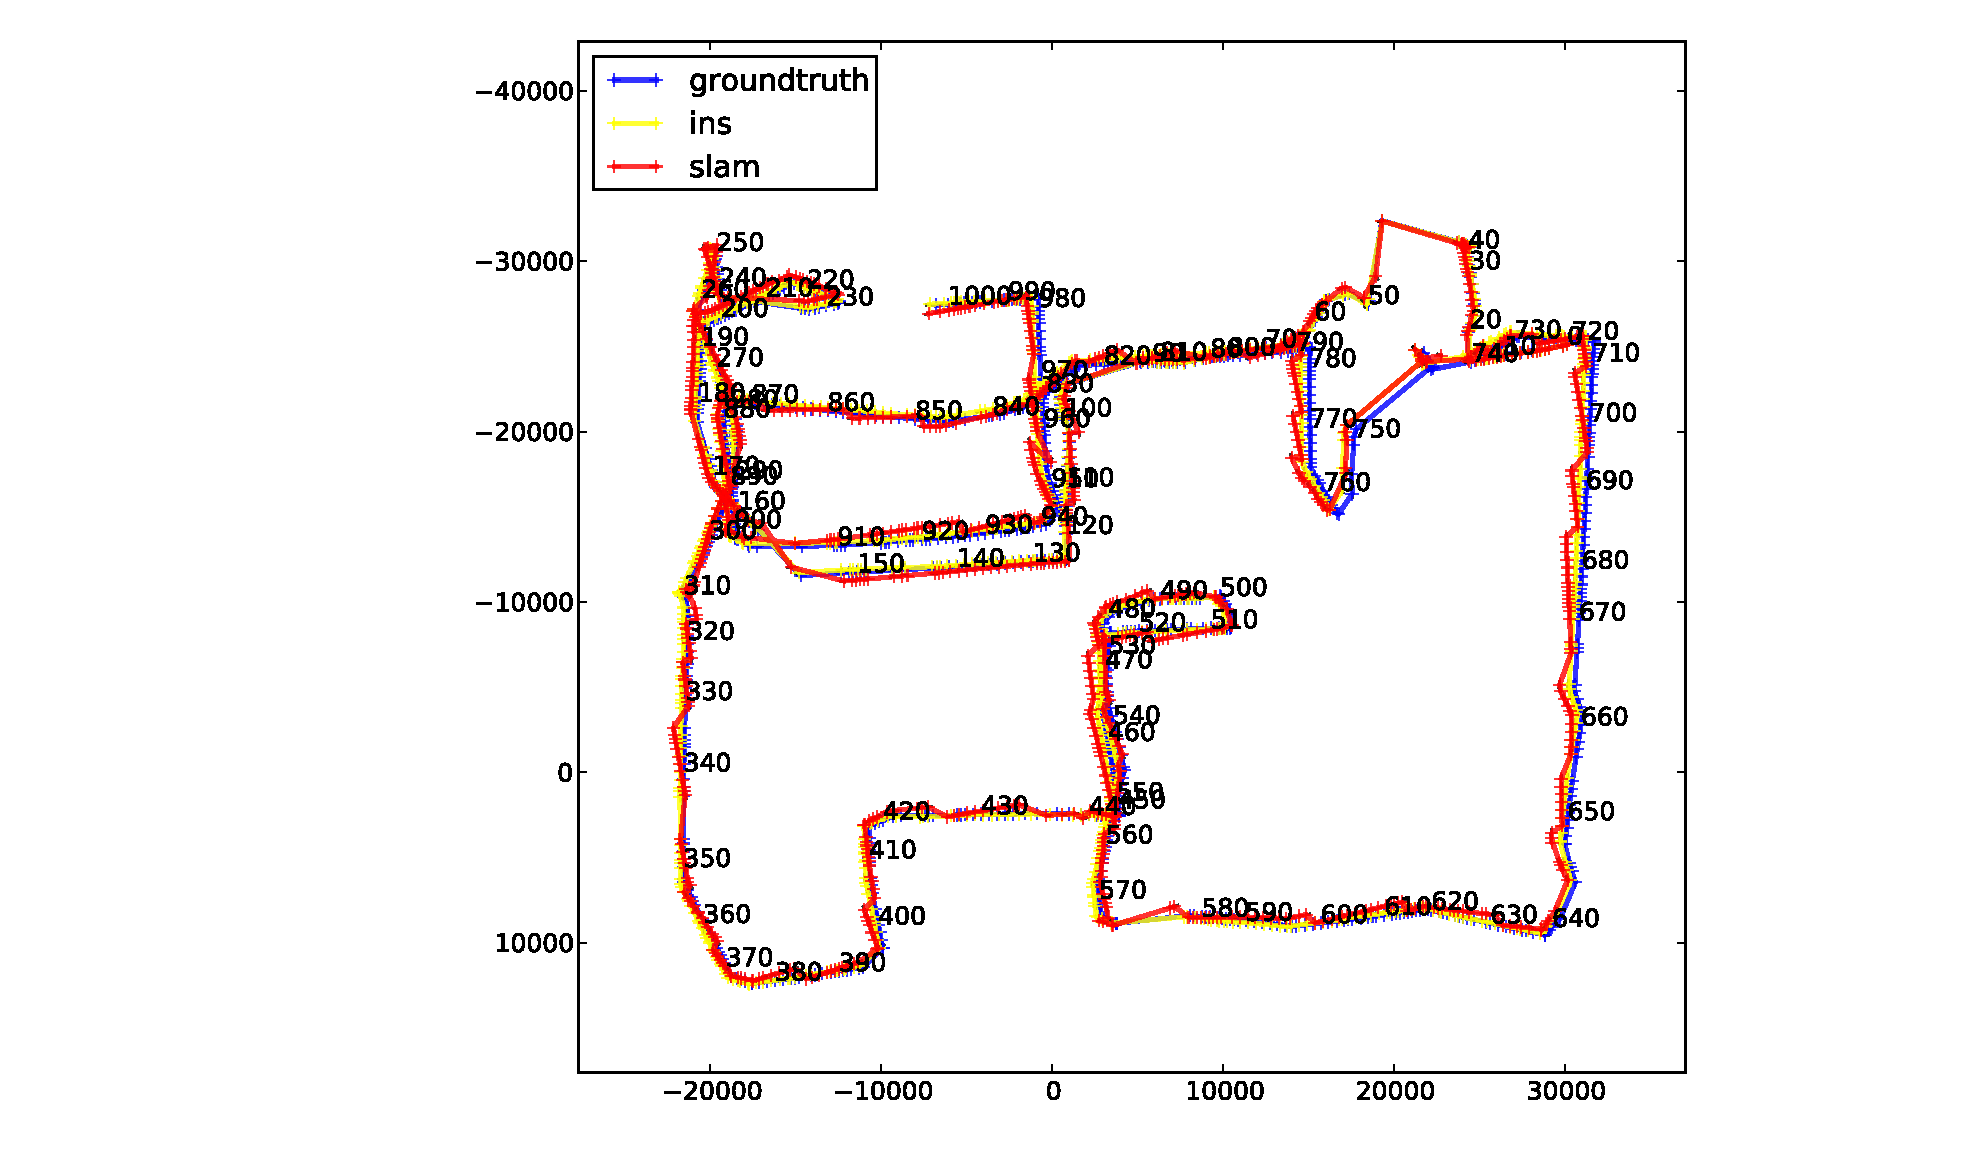
\includegraphics[width=\textwidth]{images/experiment/map3/trace2.pdf}
  \caption{The Ground Truth data, inertia sensor data and WSM slam result for map 2.}
  \label{fig:map3-trace}
\end{figure}

The error measures extracted from the Weighted Scan Matcher are shown in figure~\ref{fig:map3-confidence}. Just as in the previous experiments, there are a number of time steps where no matching scan lines were found. At these timesteps, the covariance matrix around the location estimate could not be computed, and are respresented by a red circle at the x-axis. Instead of segmenting the map at every timestep where the number of matches was zero, a different approach is tried for this experiment. The map is segmented on at those timesteps where there are 2 or more consecutive timesteps in which there were no matching scanlines. The resulting 3 submaps are shown in the appendix, figure~\ref{fig:apx:map3-pieces}.

\begin{figure}[ht]
\centering
  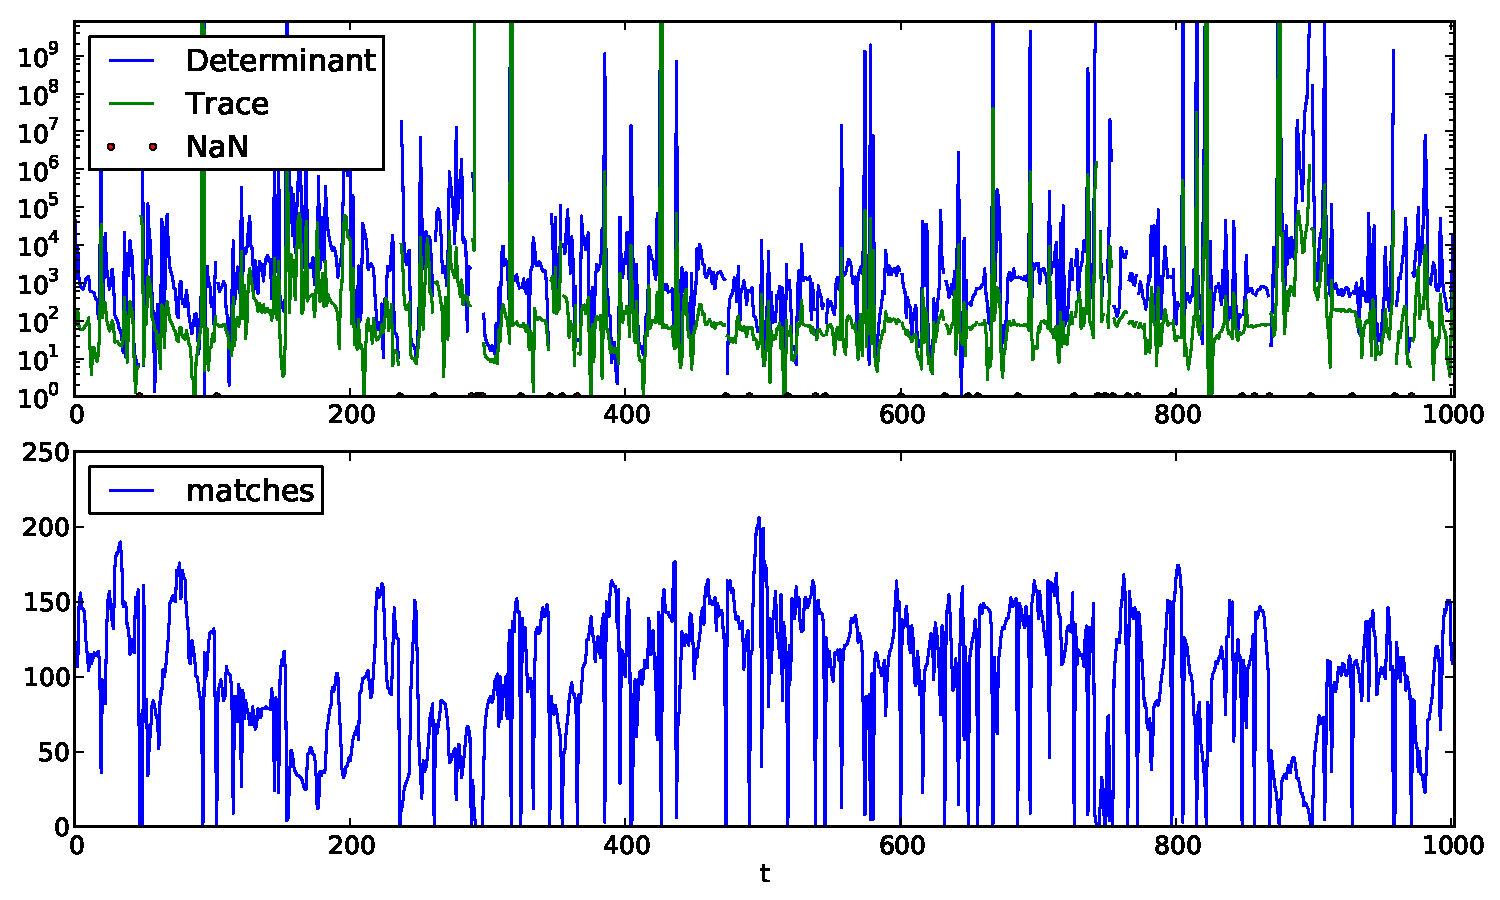
\includegraphics[width=\textwidth]{images/experiment/map3/error-measures.pdf}
  \caption{Confidence measures for map 2.}
  \label{fig:map3-confidence}
\end{figure}

The result of stitching the submaps with the Hough transform based stitching method can be inspected in figure~\ref{fig:map3-result}. As can be easily visually inspected, this result is much worse than the result by the manifold SLAM.

\begin{figure}[ht]
\centering
  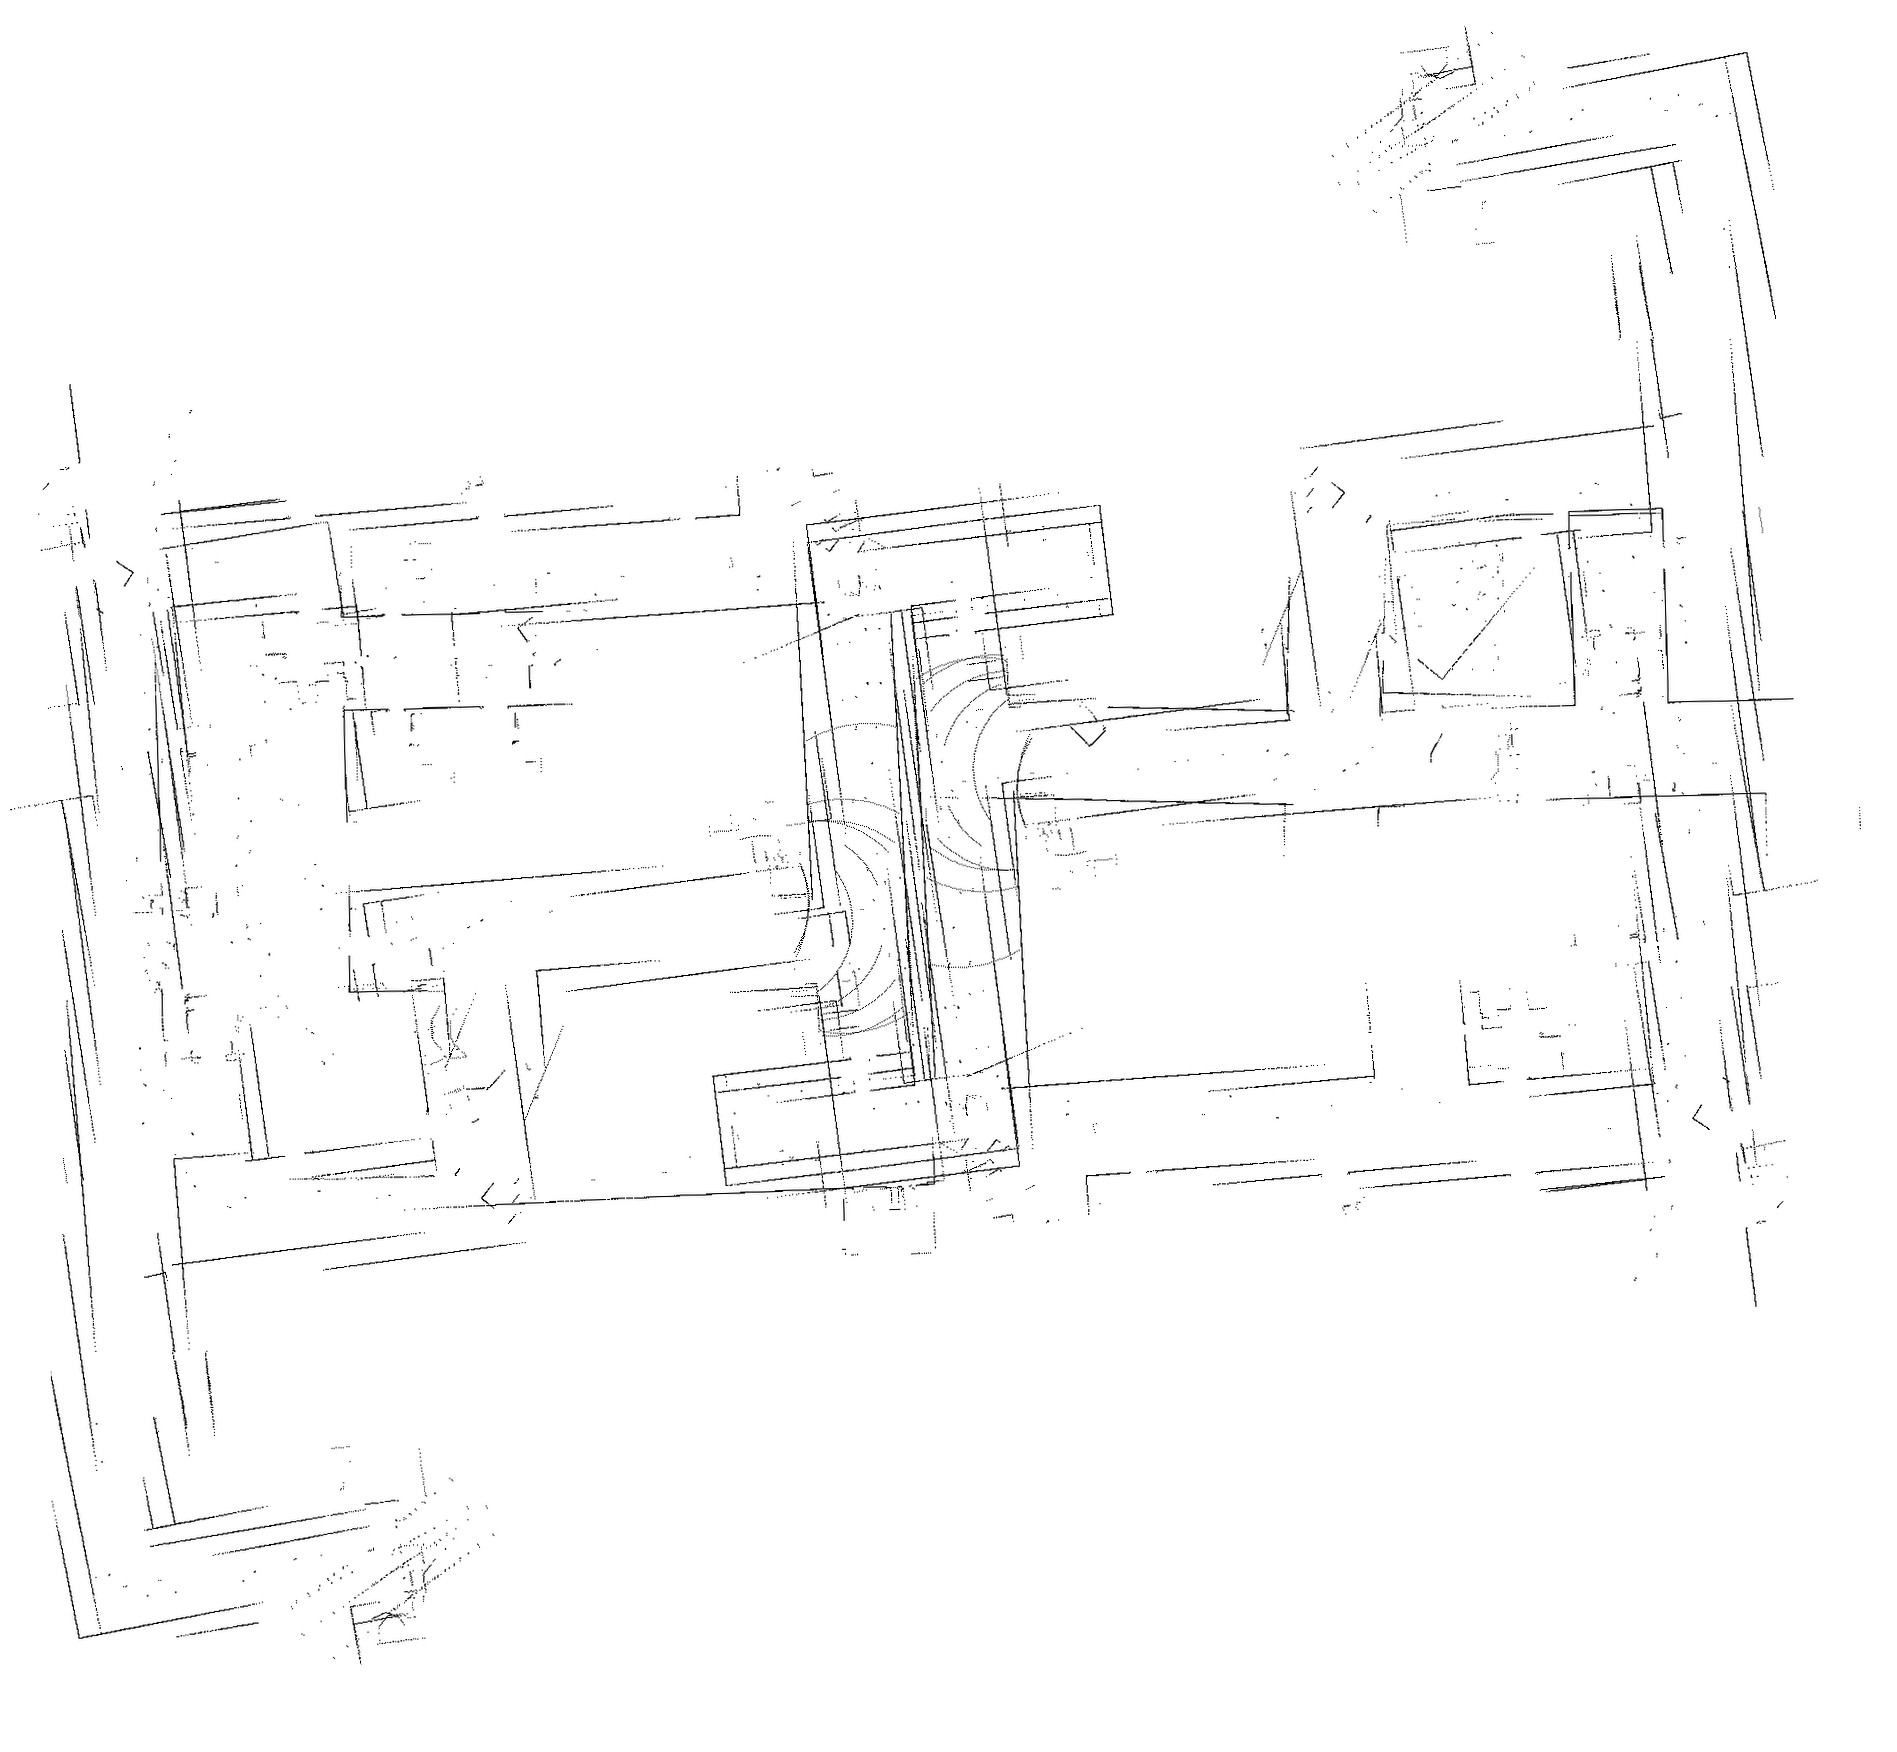
\includegraphics[width=\textwidth]{images/experiment/map3/result/step2.png}
  \caption{The resulting map after stitching all segments extracted from map 2.}
  \label{fig:map3-result}
\end{figure}

\section{Experiment 3: IranOpen 2012 Semifinal map with smoke (II)}

Due to the inferior results of the algorithm in the first two experiments, the final experiment will deviate from the first two. At the first two maps, the overlap between submaps is rather limited. For this final experiment, two maps with large overlap were created by driving the robot around in the same environment twice instead of breaking the map according to the uncertainty values. The map for this final experiment is the same as in the second experiment. The submaps are shown in figure~\ref{fig:map4-parts}. 

\begin{figure}[ht]
  \centering
  \subfigure[Piece 1]{
    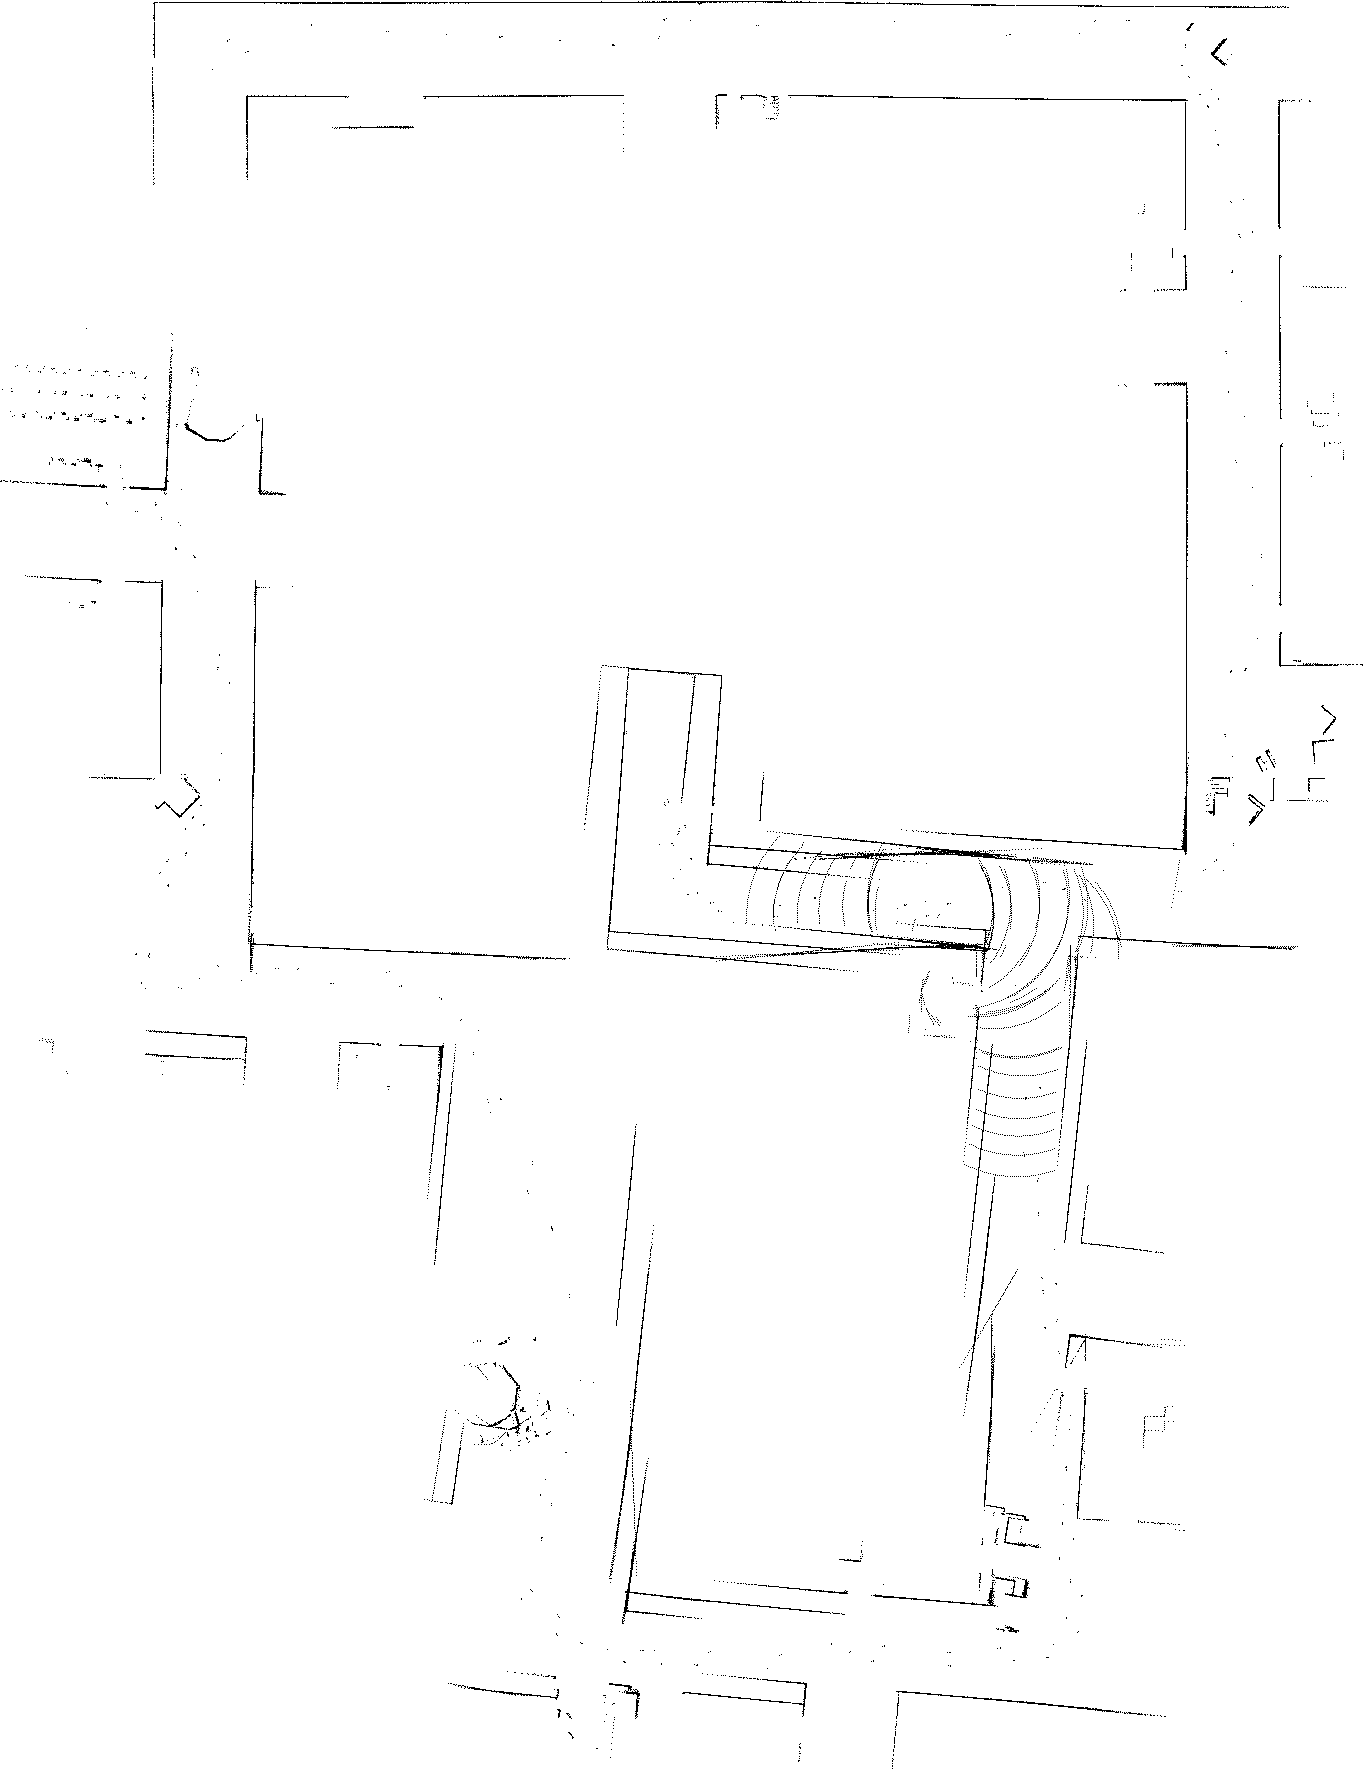
\includegraphics[width=0.45\textwidth]{images/experiment/map4/part1-1.png}
    \label{fig:map4-part1}
  }
  \subfigure[Piece 2]{
    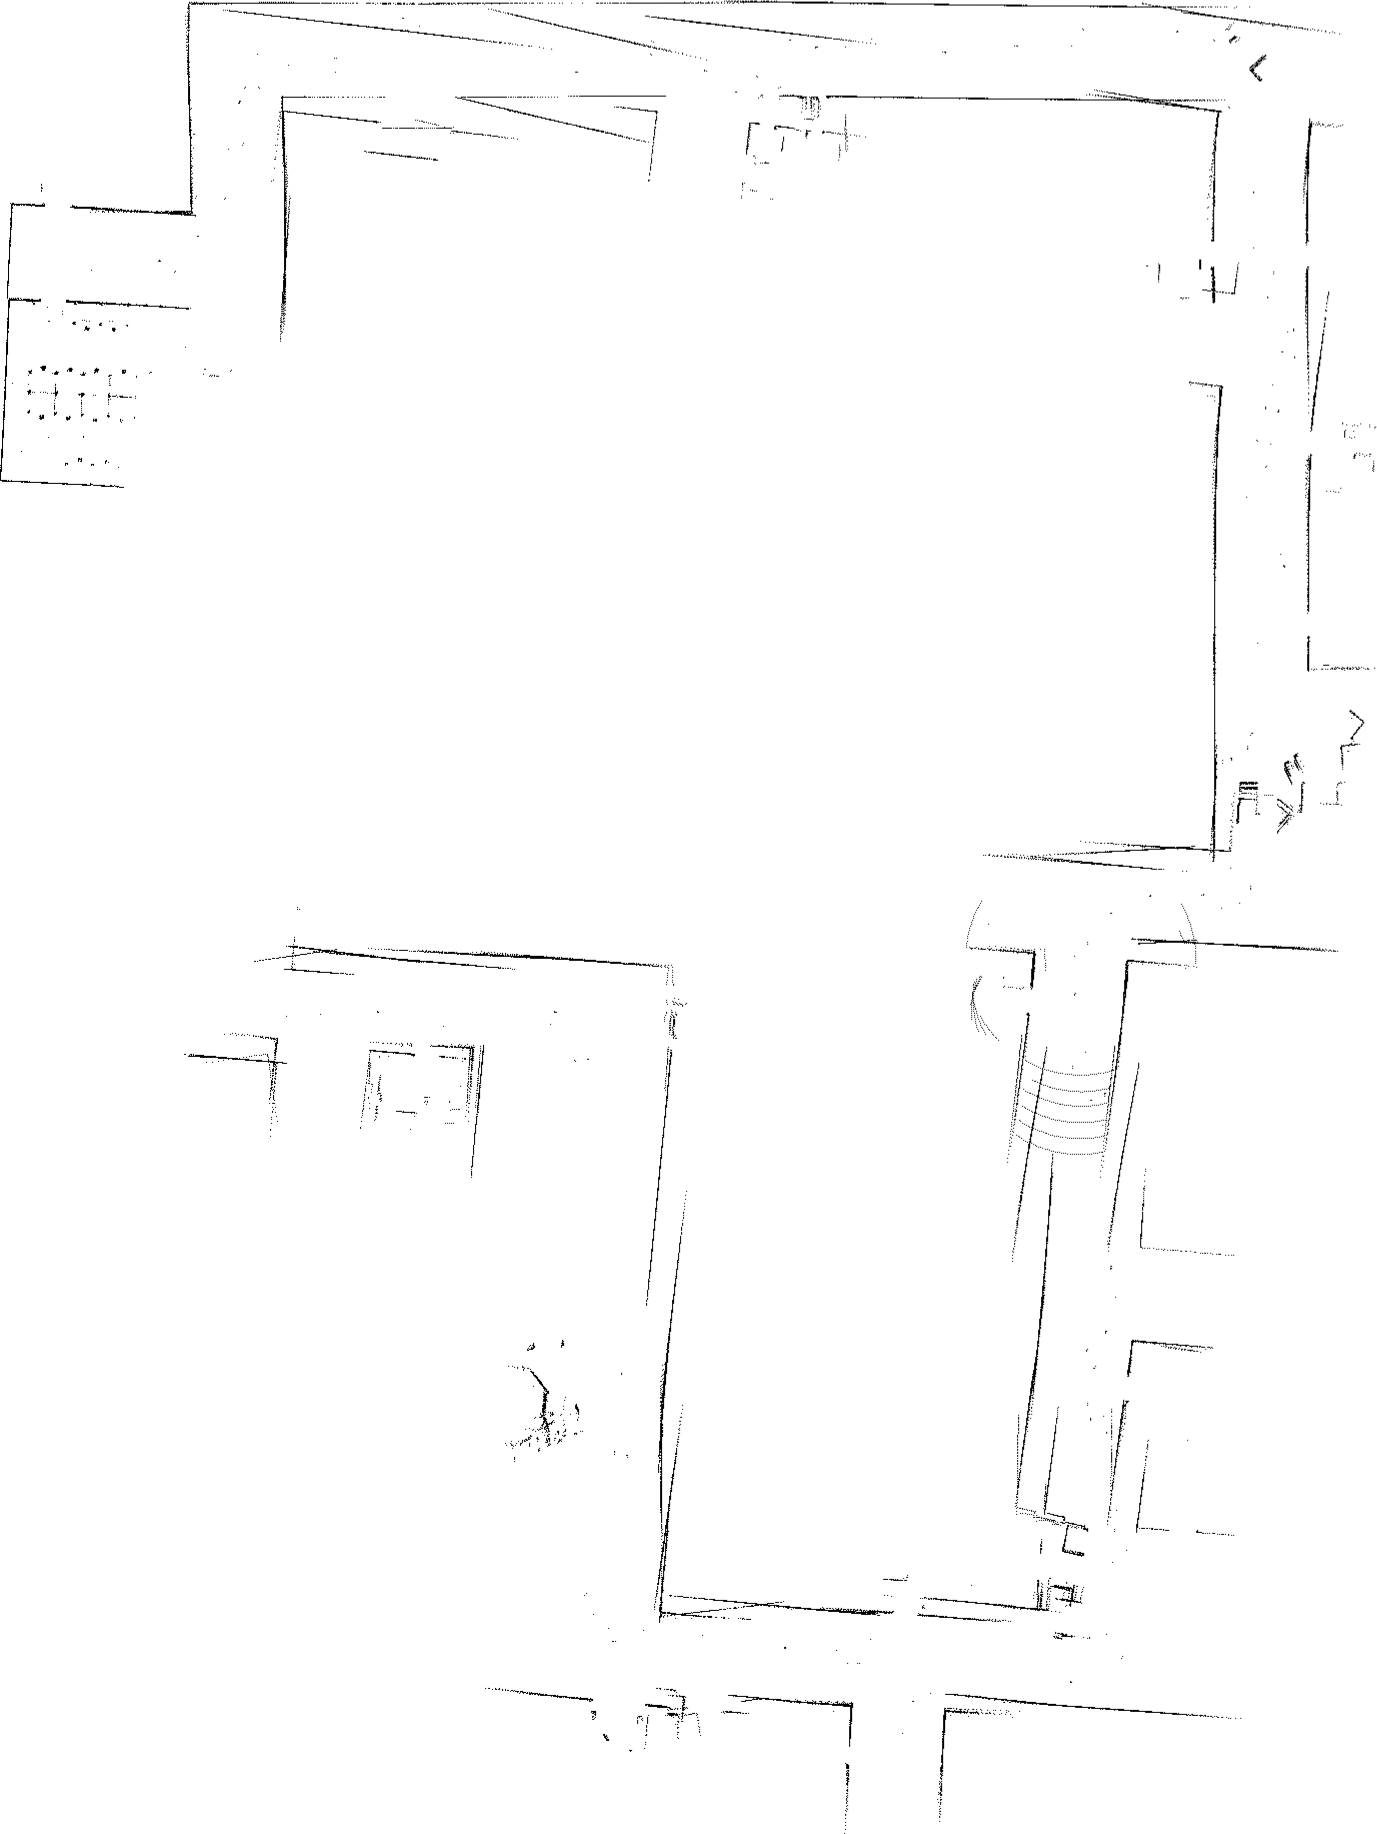
\includegraphics[width=0.45\textwidth]{images/experiment/map4/part2-1.png}
    \label{fig:map4-part2}
  }
  \caption{Map 3 pieces. The submaps overlap considerably. }
  \label{fig:map4-parts}
\end{figure}

The Hough-spectra and cross-correlation of the two maps are shown in figure~\ref{fig:map4-hough}. As expected from visual inspection of the maps, the optimal rotation $\theta$ resulting from the cross-correlation is $0\degree$. The corresponding final map is shown in figure~\ref{fig:map4-result}.

\begin{figure}[ht]
\centering
  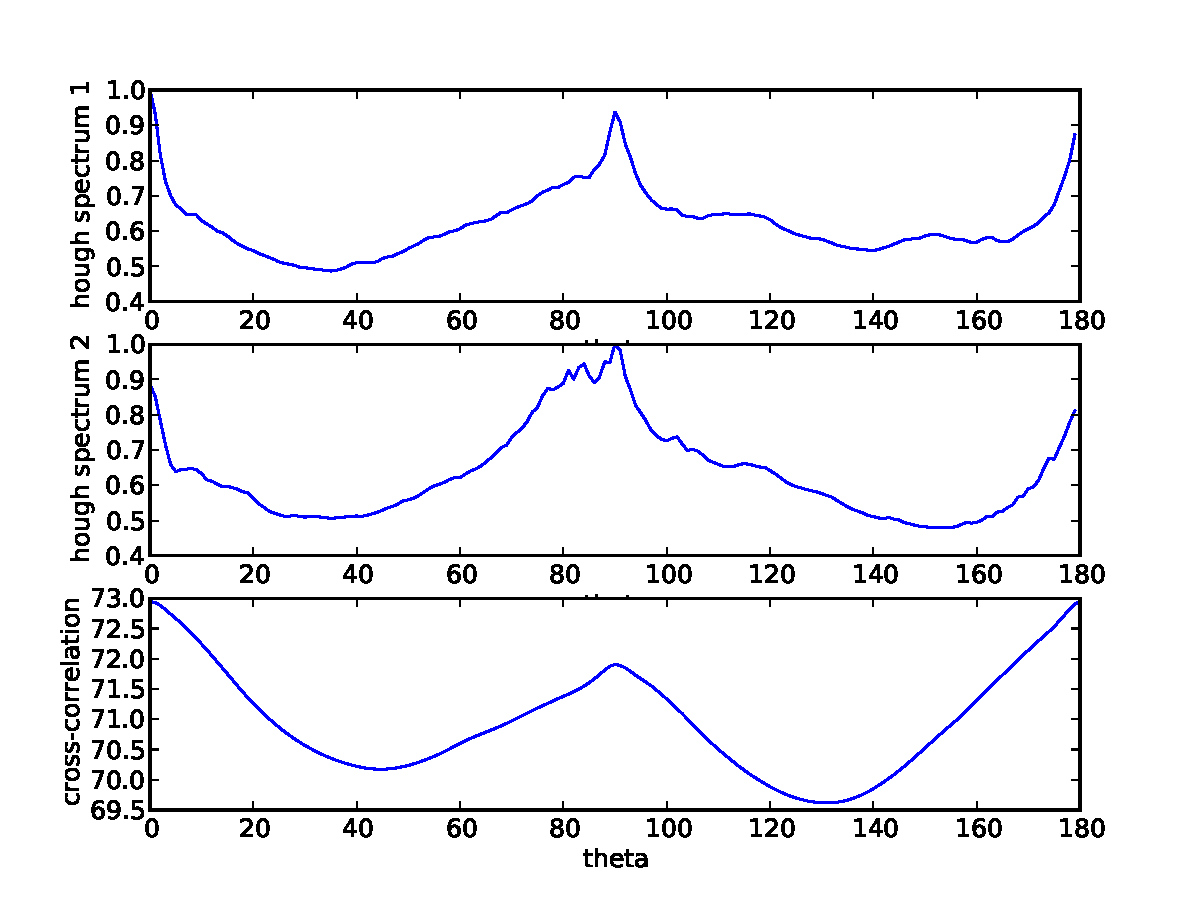
\includegraphics[width=\textwidth]{images/experiment/map4/hough.pdf}
  \caption{The Hough spectra and cross-correlation for experiment 3.}
  \label{fig:map4-hough}
\end{figure}

\begin{figure}[ht]
\centering
  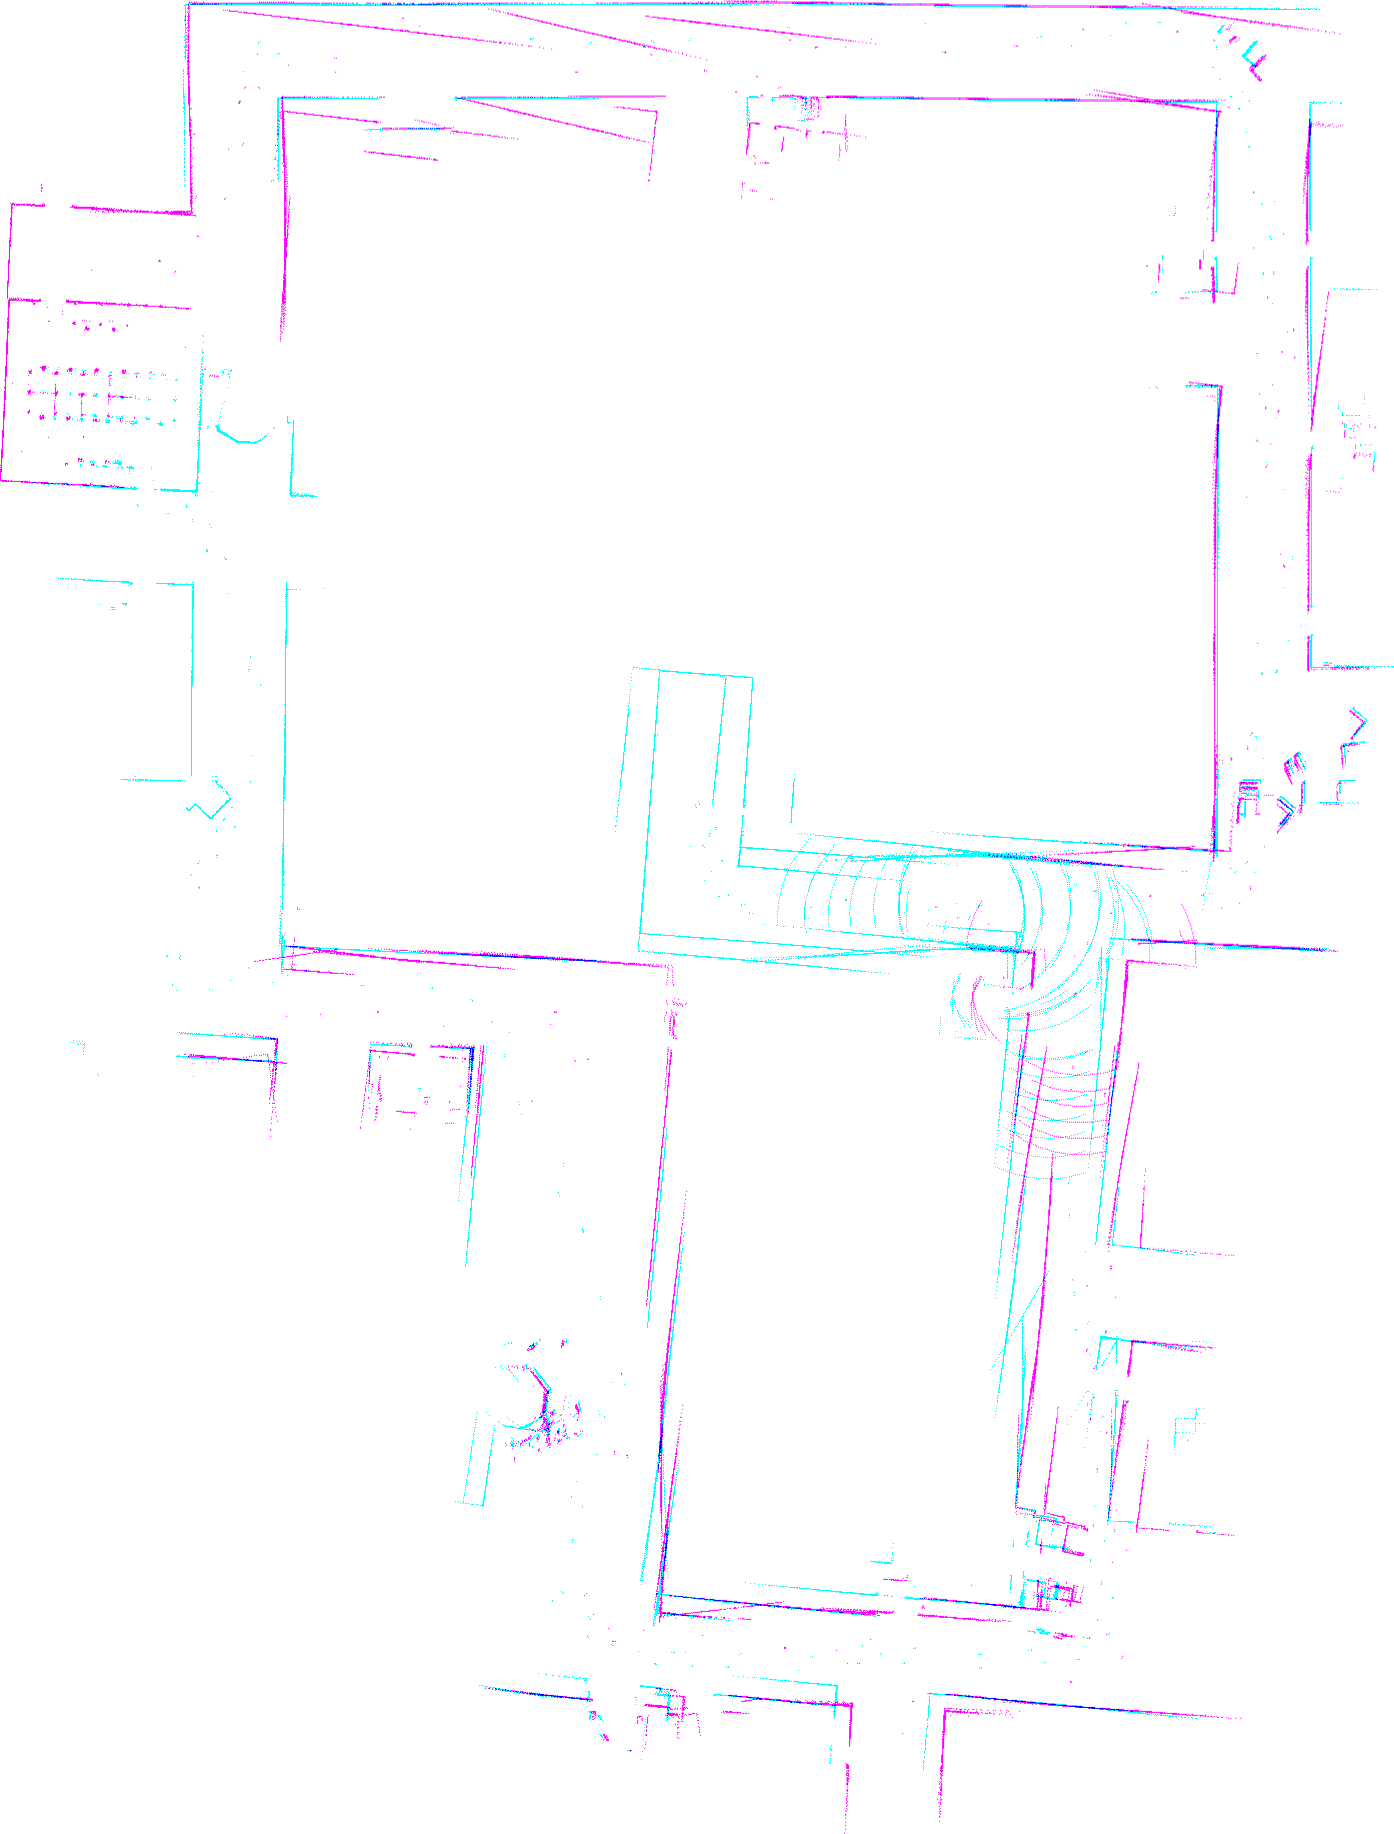
\includegraphics[width=0.55\textwidth]{images/experiment/map4/results/result_color_0.png}
  \caption{The result of Hough map stitching for experiment 3. Cyan parts are from piece 1, magenta are from piece 2. Blue parts show overlap from both pieces.}
  \label{fig:map4-result}
\end{figure}


%!TEX root = ../report.tex

%!TEX root = ../report.tex

\chapter{Future work}

Use the quad-tree based scanmatcher with a guessed initial position over the entire map.

\bibliographystyle{mystyle}
\bibliography{biblio}

\end{document}